%%%%%%%%%%%%%%%%%%%%%%%%%%%%%%%%%%%%%%%%%
% Journal Article
% LaTeX Template
% Version 1.4 (15/5/16)
%
% This template has been downloaded from:
% http://www.LaTeXTemplates.com
%
% Original author:
% Frits Wenneker (http://www.howtotex.com) with extensive modifications by
% Vel (vel@LaTeXTemplates.com)
%
% License:
% CC BY-NC-SA 3.0 (http://creativecommons.org/licenses/by-nc-sa/3.0/)
%
%%%%%%%%%%%%%%%%%%%%%%%%%%%%%%%%%%%%%%%%%

%----------------------------------------------------------------------------------------
%	PACKAGES AND OTHER DOCUMENT CONFIGURATIONS
%----------------------------------------------------------------------------------------
%[twoside,twocolumn]
\documentclass{article}

\usepackage{blindtext} % Package to generate dummy text throughout this template 
\usepackage{siunitx}
\usepackage[sc]{mathpazo} % Use the Palatino font
\usepackage[T1]{fontenc} % Use 8-bit encoding that has 256 glyphs
\linespread{1.5} % Line spacing - Palatino needs more space between lines
\usepackage{microtype} % Slightly tweak font spacing for aesthetics
\usepackage{graphicx}
\usepackage{float}
\usepackage{mathtools}
\usepackage{lineno}
\usepackage{siunitx}
\usepackage{textcomp} 




\usepackage[english]{babel} % Language hyphenation and typographical rules

\usepackage[hmarginratio=1:1,top=32mm,columnsep=20pt]{geometry} % Document margins
\usepackage[hang, small,labelfont=bf,up,textfont=it,up]{caption} % Custom captions under/above floats in tables or figures
\usepackage{booktabs} % Horizontal rules in tables

\usepackage{lettrine} % The lettrine is the first enlarged letter at the beginning of the text



\usepackage{enumitem} % Customized lists
\setlist[itemize]{noitemsep} % Make itemize lists more compact

\usepackage{abstract} % Allows abstract customization
\renewcommand{\abstractnamefont}{\normalfont\bfseries} % Set the "Abstract" text to bold
\renewcommand{\abstracttextfont}{\normalfont\small\itshape} % Set the abstract itself to small italic text

\usepackage{titlesec} % Allows customization of titles
\renewcommand\thesection{\Roman{section}} % Roman numerals for the sections
\renewcommand\thesubsection{\roman{subsection}} % roman numerals for subsections
\titleformat{\section}[block]{\large\scshape\centering}{\thesection.}{1em}{} % Change the look of the section titles
\titleformat{\subsection}[block]{\large}{\thesubsection.}{1em}{} % Change the look of the section titles

\usepackage{fancyhdr} % Headers and footers
\pagestyle{fancy} % All pages have headers and footers
\fancyhead{} % Blank out the default header
\fancyfoot{} % Blank out the default footer
\fancyhead[C]{Running title $\bullet$ May 2016 $\bullet$ Vol. XXI, No. 1} % Custom header text
%\fancyfoot[RO,LE]{\thepage} % Custom footer text

\usepackage{titling} % Customizing the title section

\usepackage{hyperref} % For hyperlinks in the PDF

\usepackage[round, comma, sort&compress]{natbib}

\setlength{\parindent}{0pt}
\setlength{\parskip}{10pt plus 1pt minus 1pt}





%----------------------------------------------------------------------------------------
%	TITLE SECTION
%----------------------------------------------------------------------------------------

\setlength{\droptitle}{-4\baselineskip} % Move the title up

\pretitle{\begin{center}\Huge\bfseries} % Article title formatting
\posttitle{\end{center}} % Article title closing formatting
\title{Reconstructing the fire history of D'urville island, and its ecological consequences} % Article title
% Your email address
%\and % Uncomment if 2 authors are required, duplicate these 4 lines if more
%\textsc{Jane Smith}\thanks{Corresponding author} \\[1ex] % Second author's name
%\normalsize University of Utah \\ % Second author's institution
%\normalsize \href{mailto:jane@smith.com}{jane@smith.com} % Second author's email address
\linenumbers
\date{\today} % Leave empty to omit a date
\renewcommand{\maketitlehookd}{%
\begin{abstract}
\noindent 
Modification of offshore island ecosystems in New Zealand began with the arrival of Polynesians c. 1280 AD. European settlement in the early 19\textsuperscript{th} century lead to further transformation. The introduction of regular burning from both waves of settlement has left lasting legacies on New Zealand's fire-sensitive native vegetation communities. D'Urville Island has a rich human history in large part because its abundance of metamorphosed indurated mudstone provided an excellent lithic resource for tool building and subsequent trade for Polynesian settlers. We analysed pollen, charcoal and magnetic susceptibility from three different locations, and developed a 2200 year record that begins c. 1550 years before human arrival, and spans c. 650 years of human occupation.  The prehuman vegetation on D'Urville Island was a heterogeneous mosaic of Nothofagaceae-\textit{Podocarpus} forest with a broadleaf sub-canopy and diverse shrub and small tree layer; a ground layer of ferns was also common.  Coastal locations and those surrounding lakes and wetlands would have been abundant in \textit{Rhopalostylis} and \textit{Dysoxylum} forest. Previous research places human settlement of D'Urville Island at c. 1500 AD (albeit with a substantial potential error range); but multiple proxy analysis from our study suggest an earlier date of c. 1300 AD. The first wave of Polynesian settlement brought with it a transformation from closed to open forest synonymous with previous paleoecological studies throughout New Zealand.  Fire was a major contributor to this transformation and charcoal is common in the record during both Polynesian and European settlement waves.  With European settlement a decline in charcoal accumulation occurs, but there is a conspicuous lack of recovery of native forest.  During this European period, exotic plant species appear and subsequently spread rapidly across the landscape.  Despite the loss of much of the closed-canopy Nothofagaceae-\textit{Podocarpus} forest, typical with much of the New Zealand mainland and offshore islands, D'Urville Island posses many areas worthy of conservation. In particular, D’Urville island supports a number of threatened mistoloe, ultramafic communities and regionally rare species.  
\end{abstract}
}

%----------------------------------------------------------------------------------------

\begin{document}

% Print the title
\maketitle

%----------------------------------------------------------------------------------------
%	ARTICLE CONTENTS
%----------------------------------------------------------------------------------------

\section{Introduction}
Anthropic changes to fire regimes have resulted in drastic and rapid shifts in ecosystem function, structure and composition, especially in locations whose ecosystems are ill-adapted to frequent fire \citep{Mcwethy2013}. New Zealand has been no exception. In comparison to a number of its Gondwanan neighbours, New Zealand's vegetation shows little evidence of adaptation to frequent fire, as fires occurred only once every 1-2 millennia prior to human settlement \cite{OgdenJ}. Infrequent fire, combined with New Zealand's maritime climate prompted \cite{OgdenJ} to suggest the pre-human frequency of fires had the potential to be millennial in some sites. \cite{Perry2014} argue that the charcoal analysis used to decipher fire frequencies is highly biased towards the east coast of the South Island, making it somewhat difficult to derive conclusions that encompass all of New Zealand. It is likely that some ecosystems experienced fire more often than others. For example, the combination of physical conditions and vegetation type in wetlands make them relatively more fire prone \citep{Perry2014,mcglone2009postglacial, McGlone1983}. Evidence from the eastern North Island suggests increasing fire activity from the mid-Holocene onwards \citep {Horrocks2001,rogers2007frequency}, possibly as a result of increasing droughts from the greater intensity and frequency of El Ni\~{n}o-Southern Oscillation (ENSO) events \citep{Perry2014, mcglone1992nino}.

Regardless of the precise fire frequencies throughout both the North and South Islands, the evidence overwhelmingly suggests that most of New Zealand's indigenous woody vegetation was not adapted to frequent fire \citep{Wilmshurst1996}. New Zealand 's tree species typically have seeds that are vulnerable to fire and lack the fire-stimulated re-sprouting capabilities of species in ecosystems where fire is more common such as much of Australia \citep{Perry2014}.  New Zealand's tree species also lack the traits fire-prone systems exhibit, such as thick bark capable of protecting cambium from lethal temperatures experienced during fires \citep{richardson2015functional}. This lack of fire-adapted vegetation, and extended period of recovery, contributed to the rapid conversion of New Zealand forest upon human arrival to open bracken-shrubland  \citep{McGlone1983}. Indeed the significant increase in bracken spores (\textit {Pteridium esculentum}) and abundance of charcoal towards the late Holocene, coinciding with the decline in forest pollen taxa, indicates increased fire frequency that accompanied Polynesian arrival \citep{McGlone1999}. A synthesis of charcoal records from 16 lakes across the South Island suggests that forest decline was both rapid and severe, reducing forest cover from 85-90\%, to as little as 40\% within 100 years \citep{McWethy2009a,mcwethy2014high}. 

To date most ecologically-oriented fire history research in New Zealand has focused on trying to understand the process and pattern of initial deforestation by human-lit fires immediately following Polynesian settlement in the 13\textsuperscript{th} century \citep { Perry2012a,Wilmshurst1996,McGlone1999,Wilmshurst2004,Wilmshurst2005,McWethy2009a}. European arrival was marked by significant changes to New Zealand landscapes yet the impact of this second wave of colonization has not been well explored.  European settlers rapidly changed the landscape. Slash and burn techniques were used to convert native bush into agriculture; however, the difficulties of controlling such fires often led to large areas of land burning unintentionally \citep{PawsonE}. Landholders were, by law, required to improve their land and to many the most efficient way to achieve this was by clearing forest with fire \citep{Salmon1975}. The combined result of both those Polynesian and European fire and deforestation footprints was a reduction of native forest to just 23\%\ of the land surface area \citep{Ewers2006}. 

The impact of European land-use during the past 1-2 centuries has been responsible for creating feedbacks leading to dramatic shifts in ecosystem dynamics, yet these more recent impacts are yet to be well examined.  The exotic flammable species that arrived with Europeans (e.g. \textit {Pinus} spp., \textit {Ulex} spp., \textit {Hakea} spp.) have helped create interesting positive fire-vegetation feedbacks \citep{Perry2014} and declines in dispersal and pollination services \citep{kitzberger2016fire,keeley2011fire}.  The introduction of seed and seedling predators \citep{perry2015exotic,sullivan2010feathers} have potentially driven landscapes into \textquotesingle{traps\textquotesingle} whereby recovery of native vegetation is severely inhibited. In the absence of intensive restoration efforts which are difficult to implement on a large scale, recovery of native vegetation is unlikely. Despite these feedbacks, interactions leading to landscape \textquotesingle{traps\textquotesingle} affecting  many parts of the North and South Island, we know little of the fire regimes and ecosystem dynamics that caused them to emerge.

Although the frequency of fire in New Zealand has declined in the late 20\textsuperscript{th} century \citep{Perry2014,anderson2008wildfires}, climate change may further challenge restoration of native forests \citep{Harris2006, Zavaleta2009,mcglone2011potential} as warmer conditions further promote fire.  Here we set out to evaluate the legacy of Polynesian and European land-use activities and the feedbacks and interactions responsible for conditions that prevent recovery and challenge restoration of native forests. We ask these questions \begin{itemize}
	\item What are the consequences of human settlement on D'Urville Island's vegetations ?
	\item Did the modification of D'Urville Island following human settlement differ to other locations in New Zealand given its archaeological significance?  
	
	\item 
\end{itemize}
and test these hypotheses x, y, z…… results provide important information for  guiding conservation and management  Better understanding of historic fire-related drivers of vegetation change will increase our fundamental knowledge of New Zealand's fire history and inform decisions when applying restoration baselines and conservation efforts in modern landscapes.  We used high-resolution pollen and charcoal reconstructions from a partially forested island in southern New Zealand to determine pre-human vegetation baselines and fire frequency. From these reconstructions we estimate Polynesian arrival and discuss the role human settlement had in shaping the modern vegetation assemblages now witnessed . We discuss the implications of such altered plant communities, while also considering the valuable conservation opportunities available.
	
\section{Study site}
D'Urville Island, Rangitoto ke te Tonga, sits at the north-western entrance to the Marlborough Sounds, South Island, New Zealand ($40^\circ$ $50'$ S $173^\circ$ $52'$ E).  At 150 km$^2$ it is New Zealand's eighth largest island.  The coastline is typical of those throughout the Marlborough sounds, and its convoluted form results from river valleys that were drowned during the post-glacial rise in sea level \citep{Wellman1962}.   Topographically the island incorporates a range of features including headlands, strong ridges, confined flats, inlets, steep hills and cliff systems.  A series of islets and rock stacks surround the island, along with several coastal lagoons \citep{Wellman1962}.  The highest point sits at 728 m (Attempt Hill) and is located close to the island's center (Fig: \ref{fig:durville}). 

\begin{figure}[H]
	\centering
	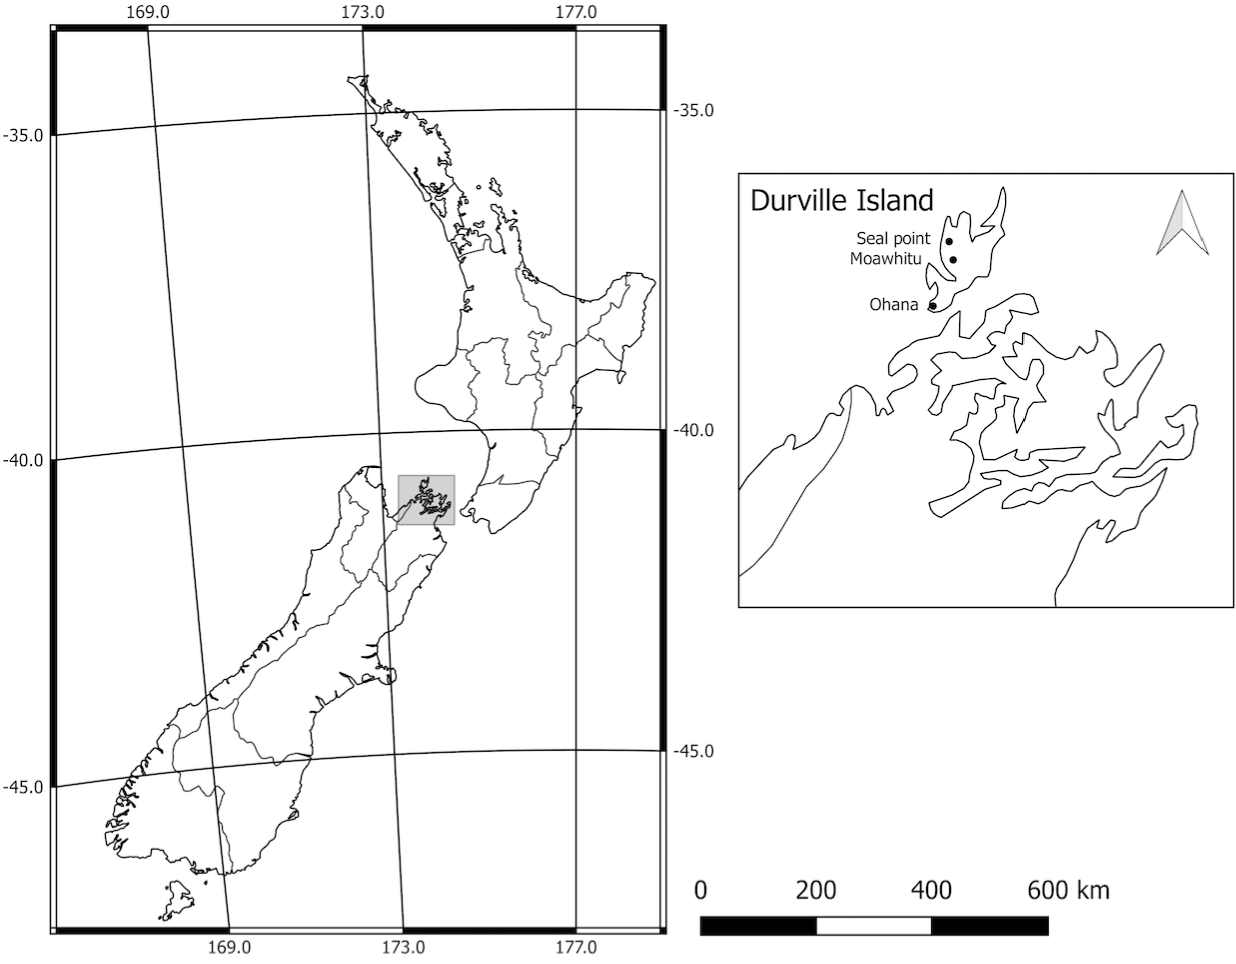
\includegraphics[scale=0.5]{figs/Durville.png}
	\caption[Location of study site (shaded)]{Location of study sites (black circles), New Zealand}
	\label{fig:durville}
\end{figure}

D'Urville's climate is maritime and consists of prevailing north-west winds, reliable rainfall, frequent gales, mild winters and warm summers \citep{walls}.  Temperatures during the summer months of January to March reach an average daily maximum of $24^{\circ}$C and are among the warmest in the South Island of New Zealand.  Typical winter daytime temperatures are in the range $10^{\circ}$C - $15^{\circ}$C.  Drought-like conditions are sometimes experienced within the region. On average, D'Urville Island receives over 1000mm of rain annually \citep{CliFlo}.

The island's geology is comprised of igneous conglomerate, Permian argillite and widespread areas of mafic and ultramafic rocks, collectively known as the \textquotesingle {Mineral Belt\textquotesingle } \citep{walls} or the \textquotesingle {Dun Mountain Ophiolite Belt\textquotesingle} \citep{lee1992new}.  As a result, the soils in parts of the island contain high concentrations of heavy metals such as iron, copper, magnesium and nickel.  Thus, it is a component of the small (0.4\%) part of the NZ landmass that can be described as \textquotesingle {serpentine\textquotesingle} \citep{lee1992new}.  The ultramafic areas create an environment difficult for most plant species, and are characterised by unique plant communities able to tolerate the high concentration of metallic minerals in the soil.  

D'Urville Island was an important cultural setting for early Polynesians.  Argillites strength and ability to hold a sharpened edge made it ideal for making weapons and tools.  Adzes, a tool dating back to the Stone Age, commonly used to smooth or carve wood, were a key instrument used for trade.  Flakes of argillite dominate the occupation layers in the cores analysed by \cite{Wellman1962}, leading him to estimate a total of 60 tonnes was extracted during the island's Polynesian occupation, or enough to manufacture not less than 15,000 adzes, acknowledging this is likely an underestimate due to the amount of flakes still hidden.  Lithic exchange was extremely important to Polynesian settlers, and we see argillites from the northern South Island appearing in the Bay of Plenty (central eastern New Zealand) less than 10 years after quarries appearing on the landscape \citep{walter2010colonisation}.  The evidence suggests that D'Urville was the centre of flourishing trade given the inferior quality of rock in other parts of New Zealand.   Midden deposits are found in every bay on D'Urville Island, as are stone walls associated with gardens \citep{walls}.  The occupation layer examined by \cite{Wellman1962} provides evidence that horticulture was likely to have been prominent on the sandy flats, as shown by the uniform distribution of pebbles associated with growing k\=umara (\textit{pomoea} spp).


The following vegetation descriptions have been summarised with permission from \cite{walls,wallsb};  other descriptions also appear in \cite{lee1992new} and \cite{beever1989new}. As with much of New Zealand, human arrival on D'Urville Island brought about a significant loss of native forest, and what remains can be best described as a complex mosaic of exotic plantations, forest remnants, pasture and areas undergoing secondary succession following clearing.  The most accessible and fertile low areas have, unsurprisingly, been converted into grazed pasture, yet areas of fernland and shrub have survived in the areas not suited to farming.  The expansion of fern and shrubland into previously grazed regions due to a cessation of farming is noticeable in several areas and these are, predictably, dominated by the early successional species such as \textit{Kunzea} spp., \textit{Leptospermum scoparium}, bracken (\textit{Pteridium esculentum}), \textit{Cyathea medullaris}, \textit{Coprosma robusta},  \textit{Melicytus ramiflorus} and  \textit{Cordyline australis}.   \textit{Fuscospora truncata} dominates on many of the ridges and slopes from 500 m above sea level (asl) to sea-level, often in association with \textit{Fuscospora solandri}, \textit{Dacrydium cupressinum} and \textit{Elaeocarpus dentatus}.  At higher elevation, and in the cooler, moister areas, \textit{Fuscospora truncata} is replaced by \textit{Lophozonia menziesii}, \textit{Lophozonia fusca}, \textit{Prumnopitys ferruginea}, \textit{Metrosideros umbellata} and other broadleaf species.  Coastal flats and some coastal slopes, along with gullies, contain many of the broadleaf species abundant throughout of the North Island of New Zealand; of these species, \textit{Dysoxylum spectabile} is most abundant, but  \textit{Rhopalostylis sapida}, \textit{Laurelia novae-zelandiae},   \textit{Beilschmiedia tawa},  \textit{Alectryon excelsus}, \textit{Piper excelsum}, \textit{Aristotelia serrata},  \textit{Hedycarya arborea}, \textit{Cyathea} spp. and \textit{Carpodetus serratus} are common.  Small examples of the low-forest climax vegetation on ultramafic areas still exist, but are limited to higher elevations and consist of \textit{Fuscospora truncata}, \textit{Dacrydium cupressinum}, \textit{Metrosideros umbellata}, \textit{Pseudopanax crassifolius} and \textit{Leptospermum scoparium}.  Although the ultramafic soils exclude many common woody weeds found in the region, wilding pines such as \textit{Pinus contorta} and \textit{Pseudotsuga menziesii} are invading some locations.  D'Urville Islands possum-free  (\textit{Trichosurus vulpecula}) status has also allowed for an abundance of mistletoe to adorn the island; also present are examples of endangered species such as {Anemanthele lessoniana} and \textit{Euphorbia glauca}.  Mammalian pests associated with much of New Zealand exist on D'Urville Island and include feral pigs (\textit{Sus scrofa}), rodents, hedgehogs (\textit{Erinaceus europaeus occidentalis}) and mustelids \citep{walls}.

%------------------------------------------------

\section{Methods}

A D-section hand corer was used to collect a 250 cm long soil core from Moawhitu Swamp.  Cores from the lakes at Seal Point (143 cm length) and Ohana (136 cm length) were collected using a simple gravity lake corer.  

\subsection{Pollen Analysis}

We subsampled 2 mL of soil from the Moawhitu Swamp core every 4 cm for pollen analysis.  Standard preparation techniques were used to make microscope slides suitable for palynological analysis \citep{moore1991pollen}. On each slide pollen from trees, shrubs, herbs and bracken spores were recorded until a total of 250 grains was reached.  Reference collections (Landcare Research) and atlases \citep[e.g.][]{moar1993pollen} were used to identify pollen to the highest possible taxonomic resolution. Distinct and unprecedented changes in vegetation and charcoal inputs were used to isolate initial human activity. Pollen and charcoal diagrams were constructed using the C2 software package \citep{juggins2003software}

\subsection{Charcoal Analysis}

Charcoal was examined at high-resolution as per \cite{whitlock2002charcoal} to reconstruct local fire activity. Samples from Moawhitu Swamp, Seal Point and Ohana cores were taken at contiguous 1 cm intervals using a brass sampler with a rectangular cutting edge.  Sub-samples were taken at a volume of 2 cm$^{3}$ where sufficient material was available, and 1 cm$^{3}$ if not in the Moawhitu Swamp core. At both Seal Point and Ohana sub-samples were taken at a volume of 5 cm$^{3}$. All samples were soaked in 6\% bleach for 24 hours. At Moawhitu Swamp samples were washed through Petri dishes 250 \si{\micro\metre}, 125 \si{\micro\metre} and 63 \si{\micro\metre}, at Seal Point and Ohana samples were washed through 125 \si{\micro\metre} Petri dishes. Charcoal particles were counted using a stereomicroscope at 50-100x magnification. Charcoal concentration (number of particles/cm$^{3}$) was determined using total charcoal counts divided by the volume of sediment sieved. Charcoal accumulation rates were calculated by dividing charcoal concentration by deposition time (yr/cm) between each sample. 


\subsection{Radiocarbon dating}

We submitted three twig samples from the Moawhitu Swamp core to the Waiakto Radiocarbon
Dating Laboratory, New Zealand for accelerator mass spectrometry (AMS) radiocarbon dating.
Ages of all dated material are expressed as calibrated $^{14}$C age before present (cal. year
BP). The samples from Moawhitu Swamp were taken from 32 cm, 59 cm and 94 cm.
Three cal. year BP dates were supplied from Ohana at 94 cm, 103 cm and 122 cm,
and three from Seal Point at 80 cm, 105 cm and 115 cm. These dates are courtesy of
Dr. David McWethy, Montanta State University, USA. Age-depth modelling, as per the
algorithm of \citep{haslett2008simple} and the Southern Hemisphere (SHCal13) calibration
curve \citep{hogg2013shcal13}, were constructed using the Bchron package \citep{parnell2014bchron} in the R statistical suite \citep{R-stat} version 3.1.3 (Fig: \ref{fig:age-depth-model}).

\begin{figure}[H]
	\centering
	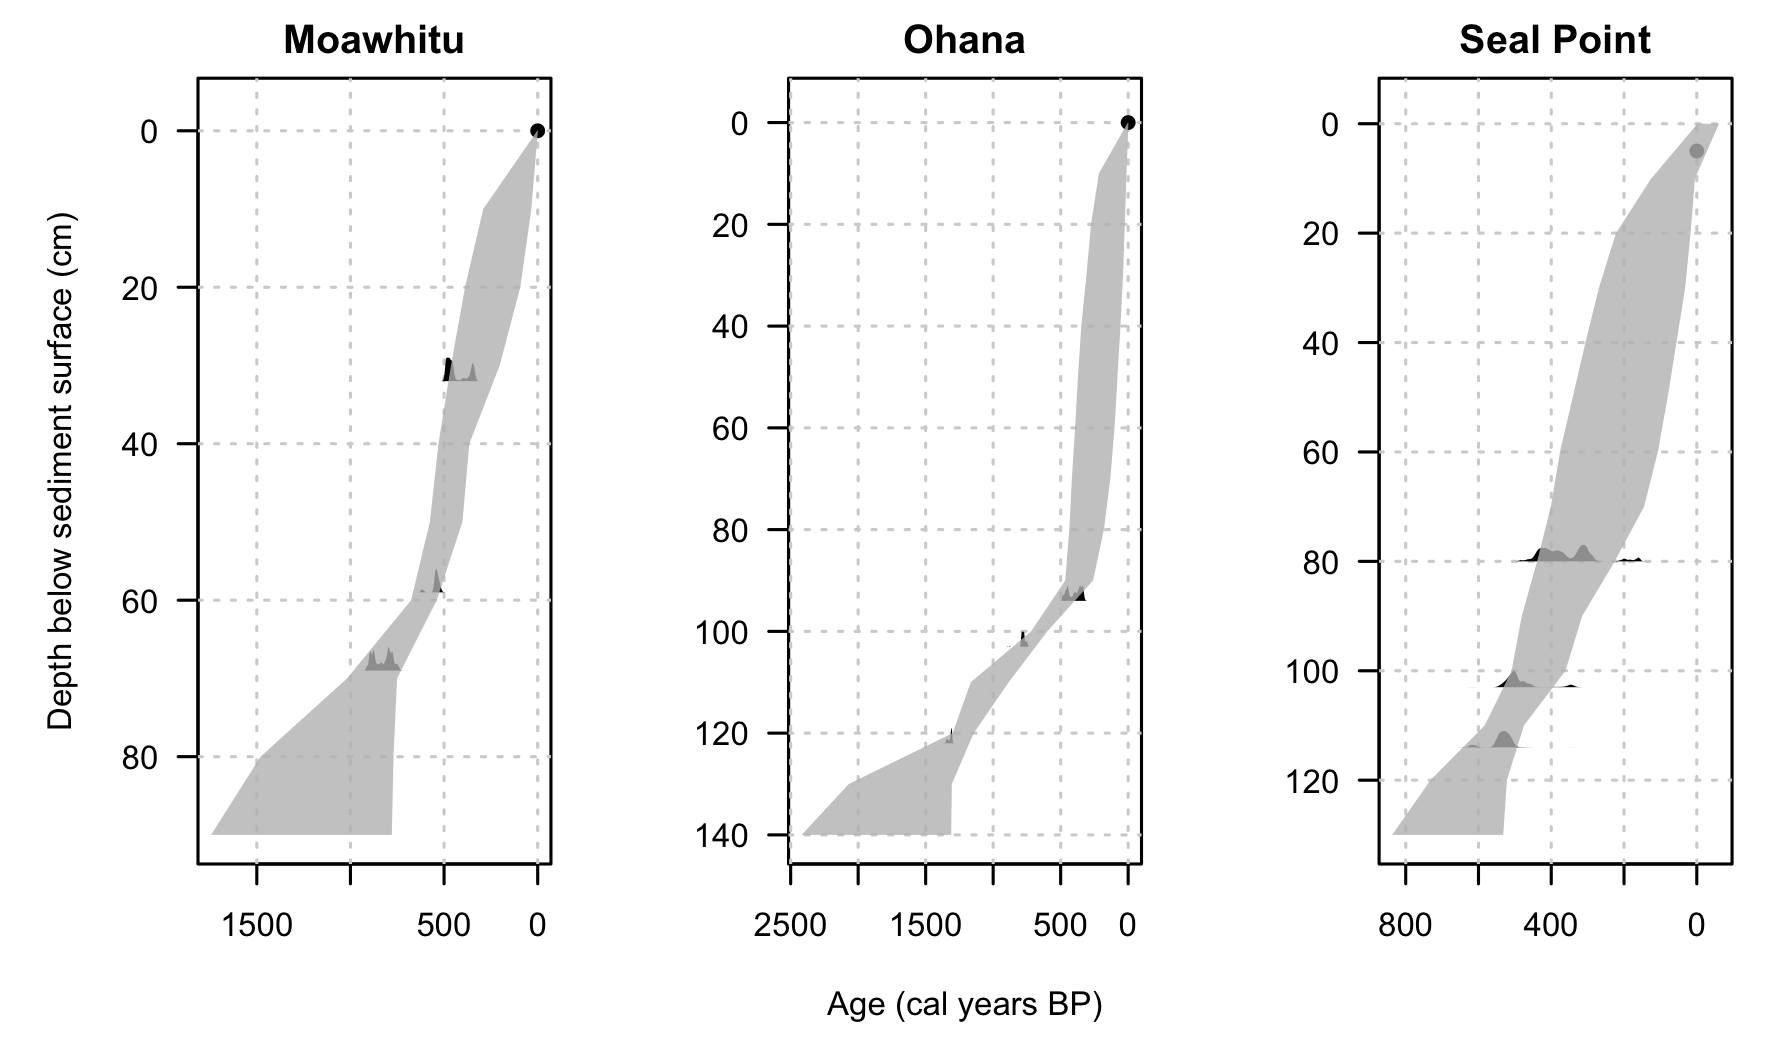
\includegraphics[scale=0.25]{Figs/age-depth-models/age-depth-model-all.png}
	\caption{Age depth models for each site constructed using the compound Poisson-Gamma chronology model of \cite{haslett2008simple}. Light grey distributions indicate probability distributions from calibrated $^{14}$C dates.}
	\label{fig:age-depth-model}
\end{figure}

\subsection {Statistical analysis}
Statistical analysis was conducted using the R statistical package \citep{R-stat}, version 3.2.3.  Constrained cluster analysis that honoured the location of sites (CONISS), and nMDS ordination, using the Bray-Curtis measure \citep{faith1987compositional} were performed on the pollen reconstruction from Moawhitu Swamp using the rioja \citep{rioja} and VEGAN \citep{dixon2003vegan} packages. Permutational multivariate analysis of variance (PERMANOVA) using distance matrices \citep{anderson2001new} were performed using the adonis command to statistically evaluate the dissimilarity between settlement and prehuman zones. Temporal auto-correlation between charcoal and magnetic susceptibility was conducted using the acf and ccf functions. 

\subsection {Magnetic Susceptibility}
Not sure of the methods here.... Only for Seal Point and Ohana


%------------------------------------------------

\section{Results}

The timing of human arrival was estimated using a combination of distinct changes
in pollen taxa (e.g. the introduction of exotic species), charcoal reconstructions and
accompanied by statistical analysis of the pollen reconstruction from Moawhitu Swamp.  Three zones were initially
identified as a result of nMDS ordination on pollen taxa from the Moawhitu Swamp core: Zone 3 (0-20 cm, 0-125 cal.
years BP), zone 2 (20-64 cm, 150-650 cal. years BP) and zone 1 (64-250 cm, 650-2200
cal. years BP) (Fig: \ref{fig:ordination}). Vegetation changes are demonstrated by a rapid rise in bracken
and Poaceae, accompanied by a decrease in native forest taxa (Fig: \ref{fig:podo-beach-tree}, \ref{fig:ferns}, \ref{fig:disturbance}), and the increase of charcoal
into the Moawhitu Swamp, Seal Point and Ohana cores (Fig: \ref{fig:podo-beach-tree}, \ref{fig:charcoal-ohana}, \ref{fig:charcoal-seal}). 



\begin{figure}[H]
	\centering
	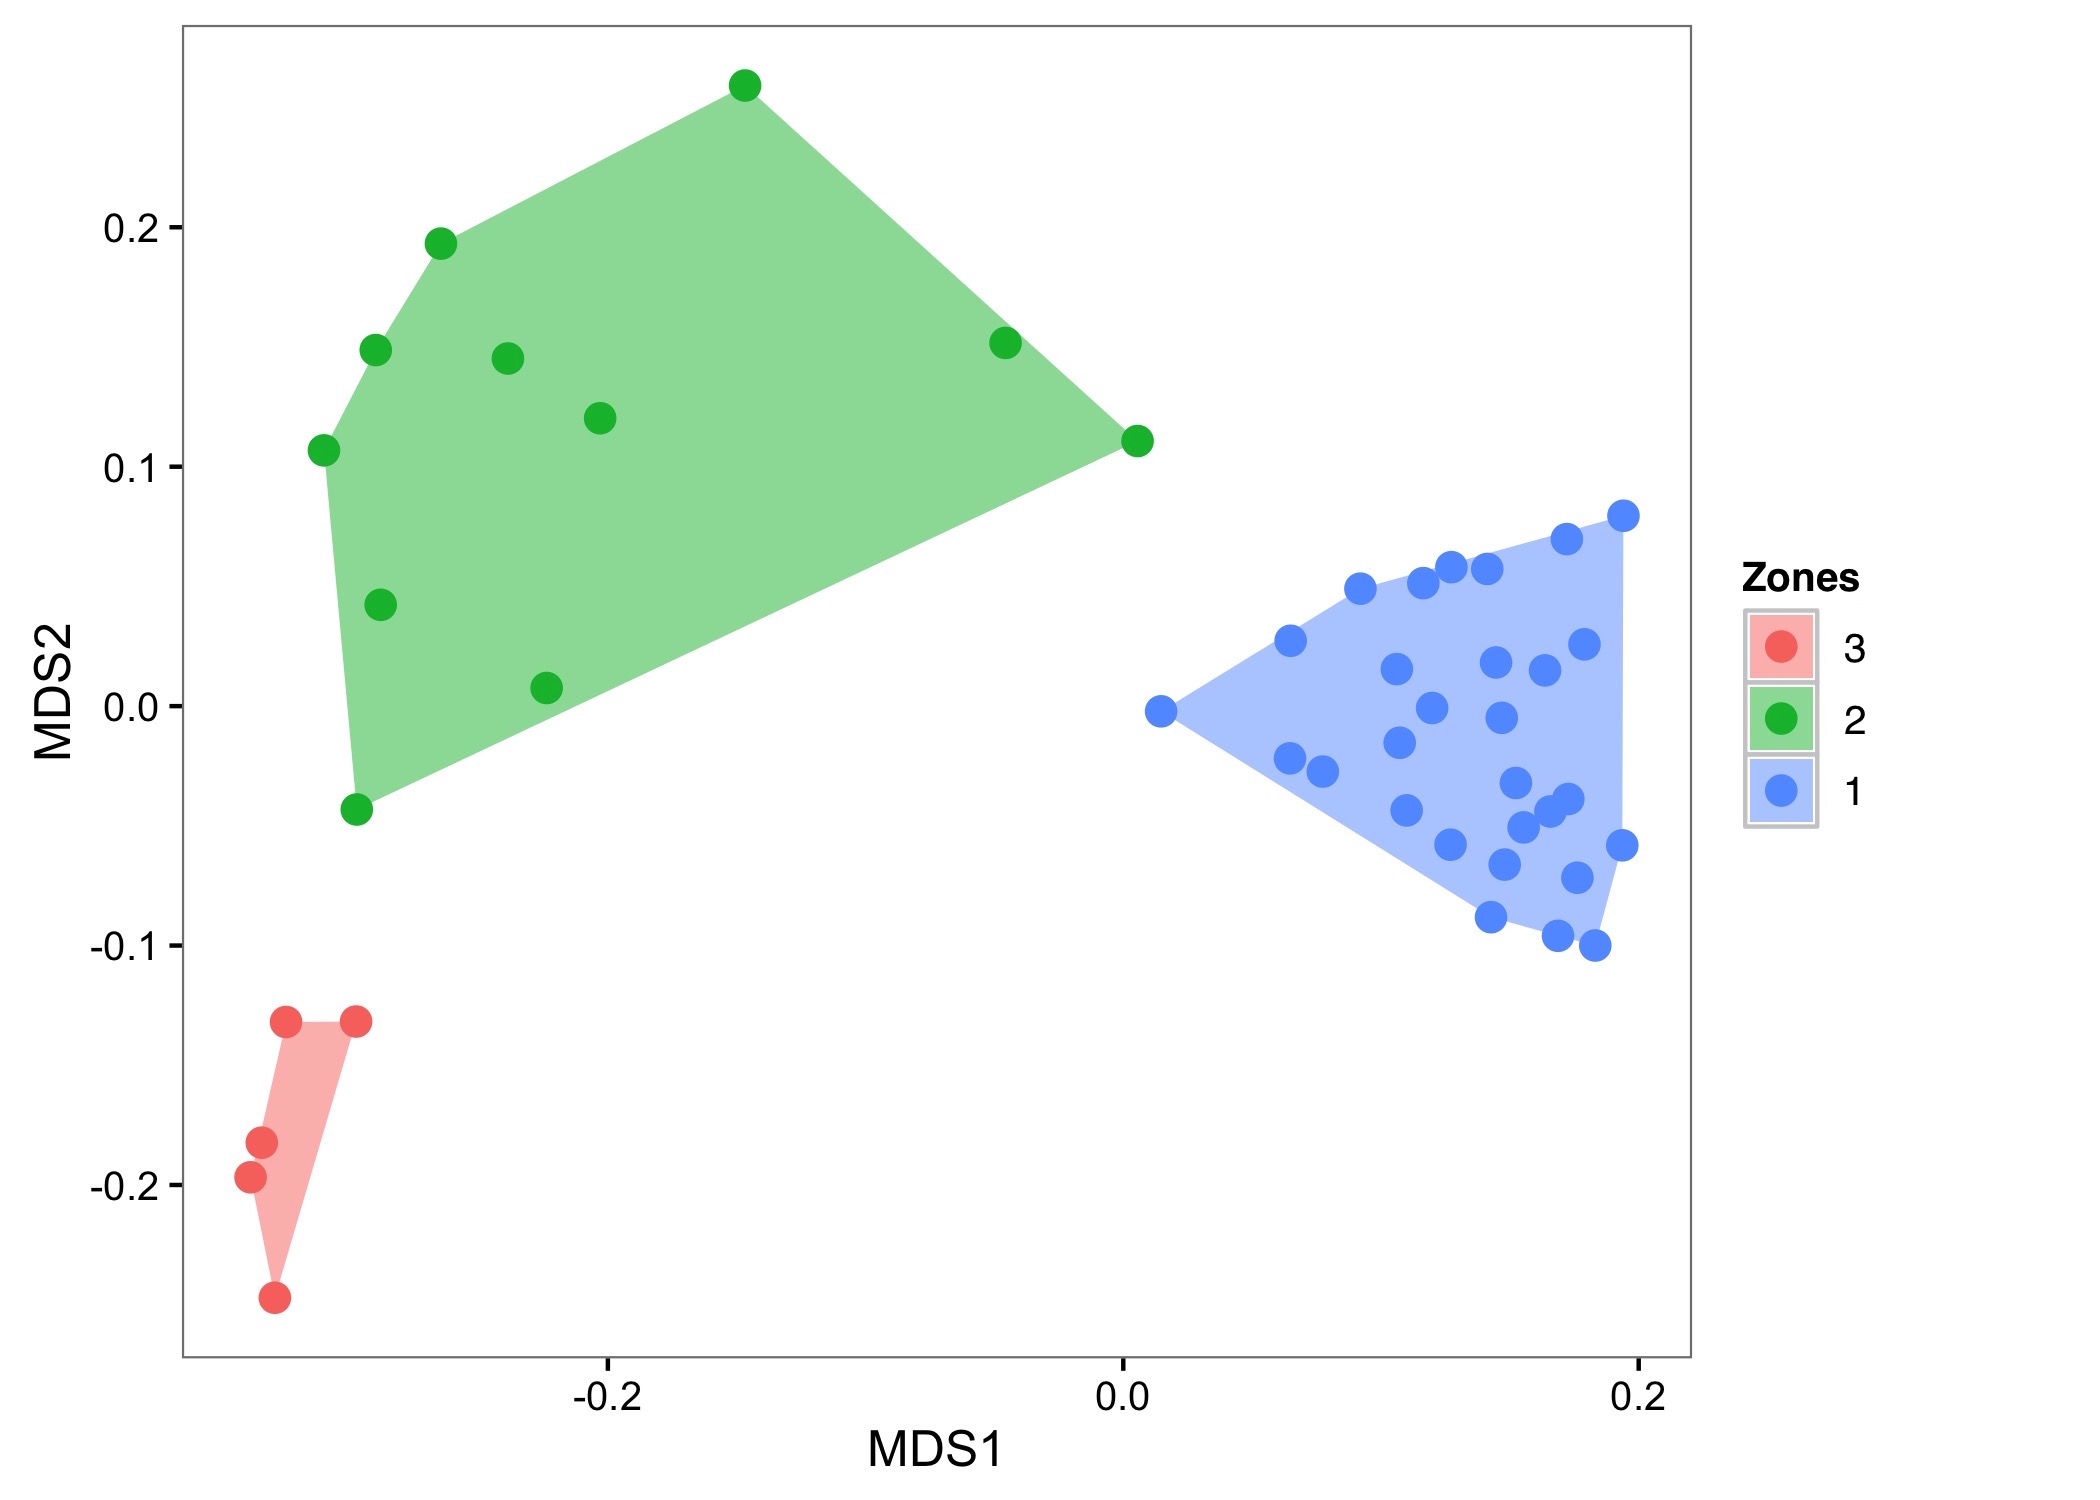
\includegraphics[scale=0.20]{Figs/nmds-analysis.jpeg}
	\caption{nMDS Ordination of settlement and prehuman zones identified from cluster analysis.  Zones identified by different colors.  Stress level = 0.1.  Polygons indicate minimum bounding box.}
	\label{fig:ordination}
\end{figure}

 

\subsection{Zone 1 - 650 - 2120 cal. years BP}
Based on the pollen present, zone 1 comprises a Nothofagaceae-\textit{Podocarpus} mosaic with a broadleaf sub-canopy and a ground layer of ferns (Fig: \ref{fig:podo-beach-tree}, \ref{fig:ferns}).  Also notable is the presence of \textit{Rhopalostylis sapida} and \textit{Dysoxylum spectabile}, which is indicative of a rich coastal, lake and wetland forest.  There are no discernible shifts in vegetation during this part of the core and pollen sum percentages remain relatively consistent.  The podocarp taxa are the most variable component of the palynoflora (Fig: \ref{fig:podo-beach-tree}). 

\begin{figure}
	\centering
	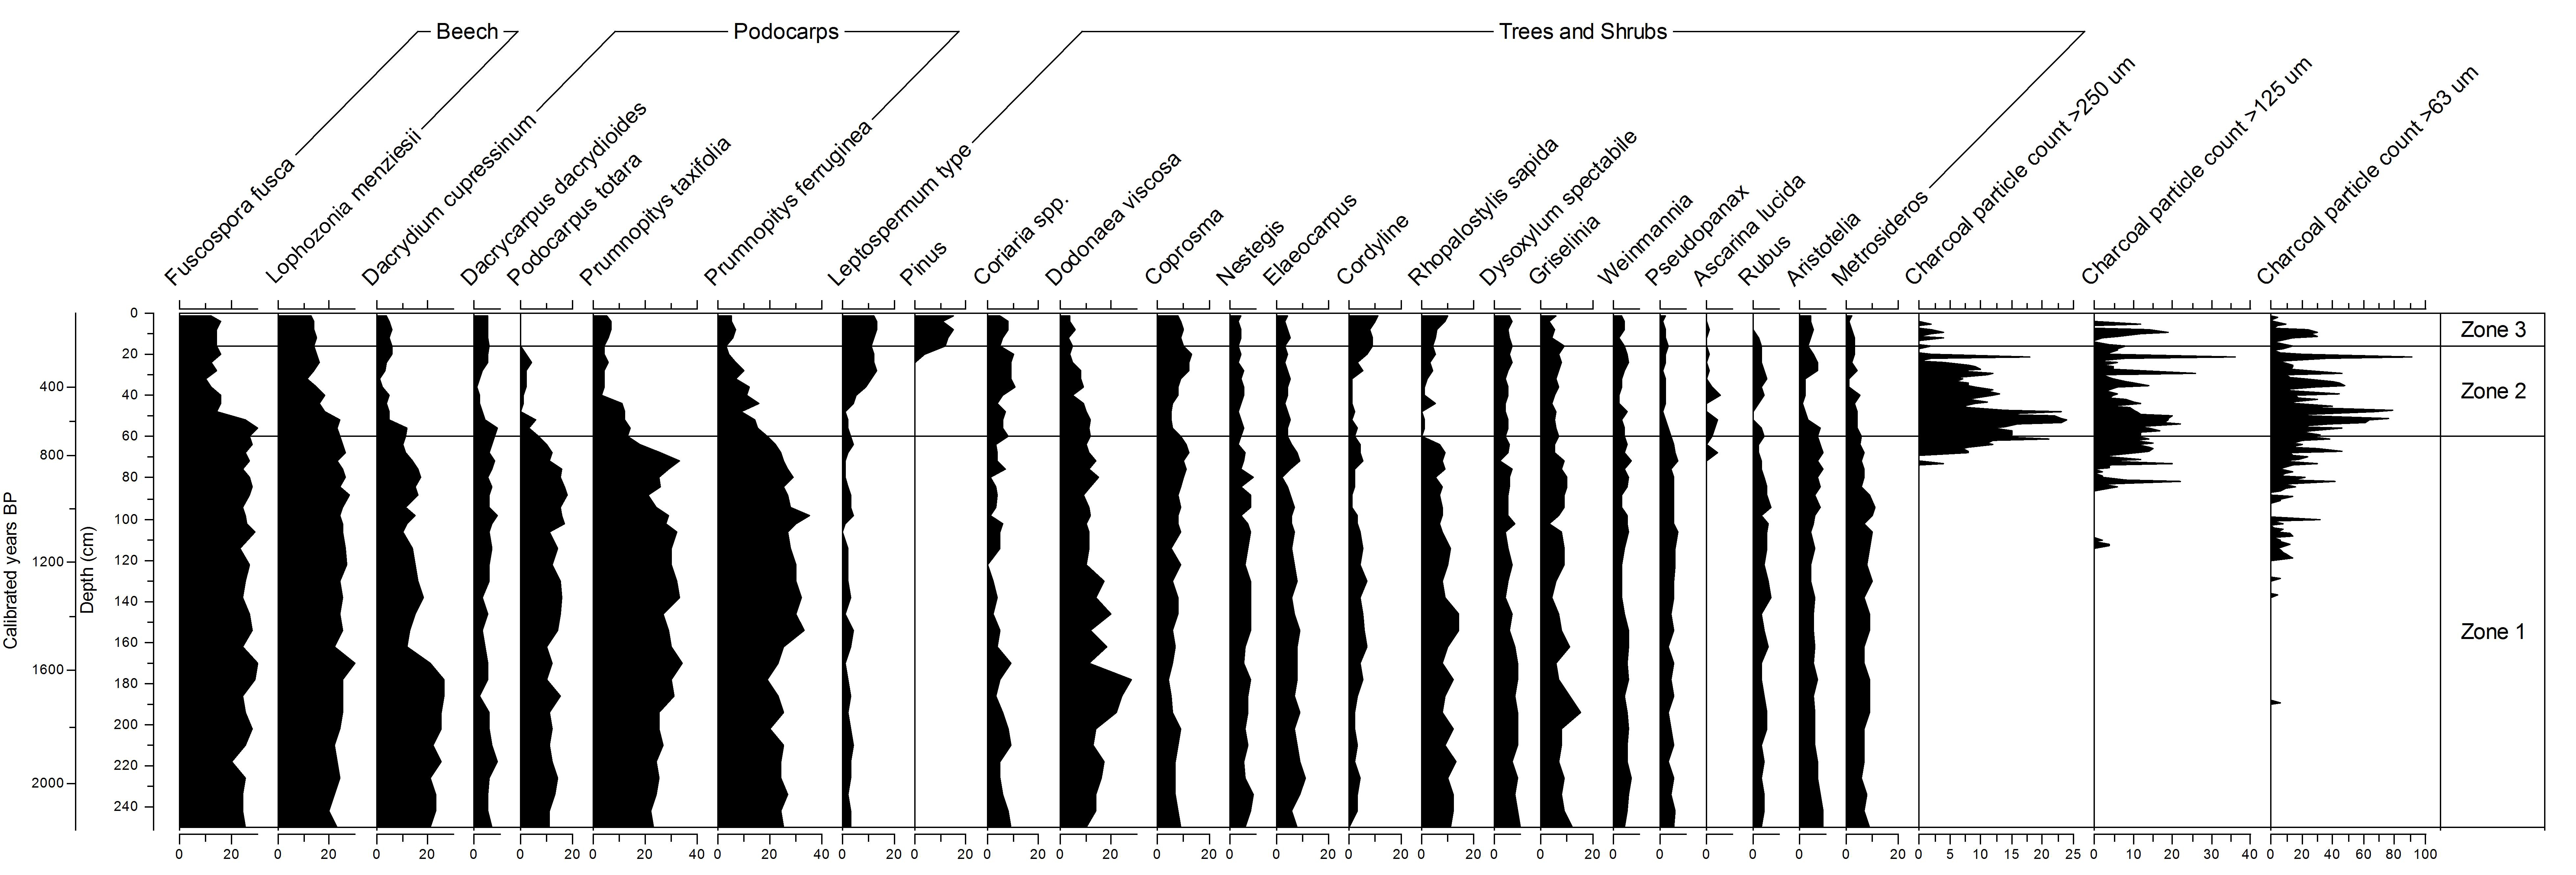
\includegraphics[scale=0.07, angle =90]{trees-shrubs-zone-corrected.jpg}
	\caption[\textit{Nothofagaceae}, \textit{Podocarpaceae} and small trees and shrubs identified at Moawhitu Swamp]{\textit{Nothofagaceae}, \textit{Podocarpaceae} and small trees and shrubs pollen identified at Moawhitu Swamp.  Pollen sum given as a percentage of total pollen count.}
	\label{fig:podo-beach-tree}
\end{figure}

\begin{figure}
	\centering
	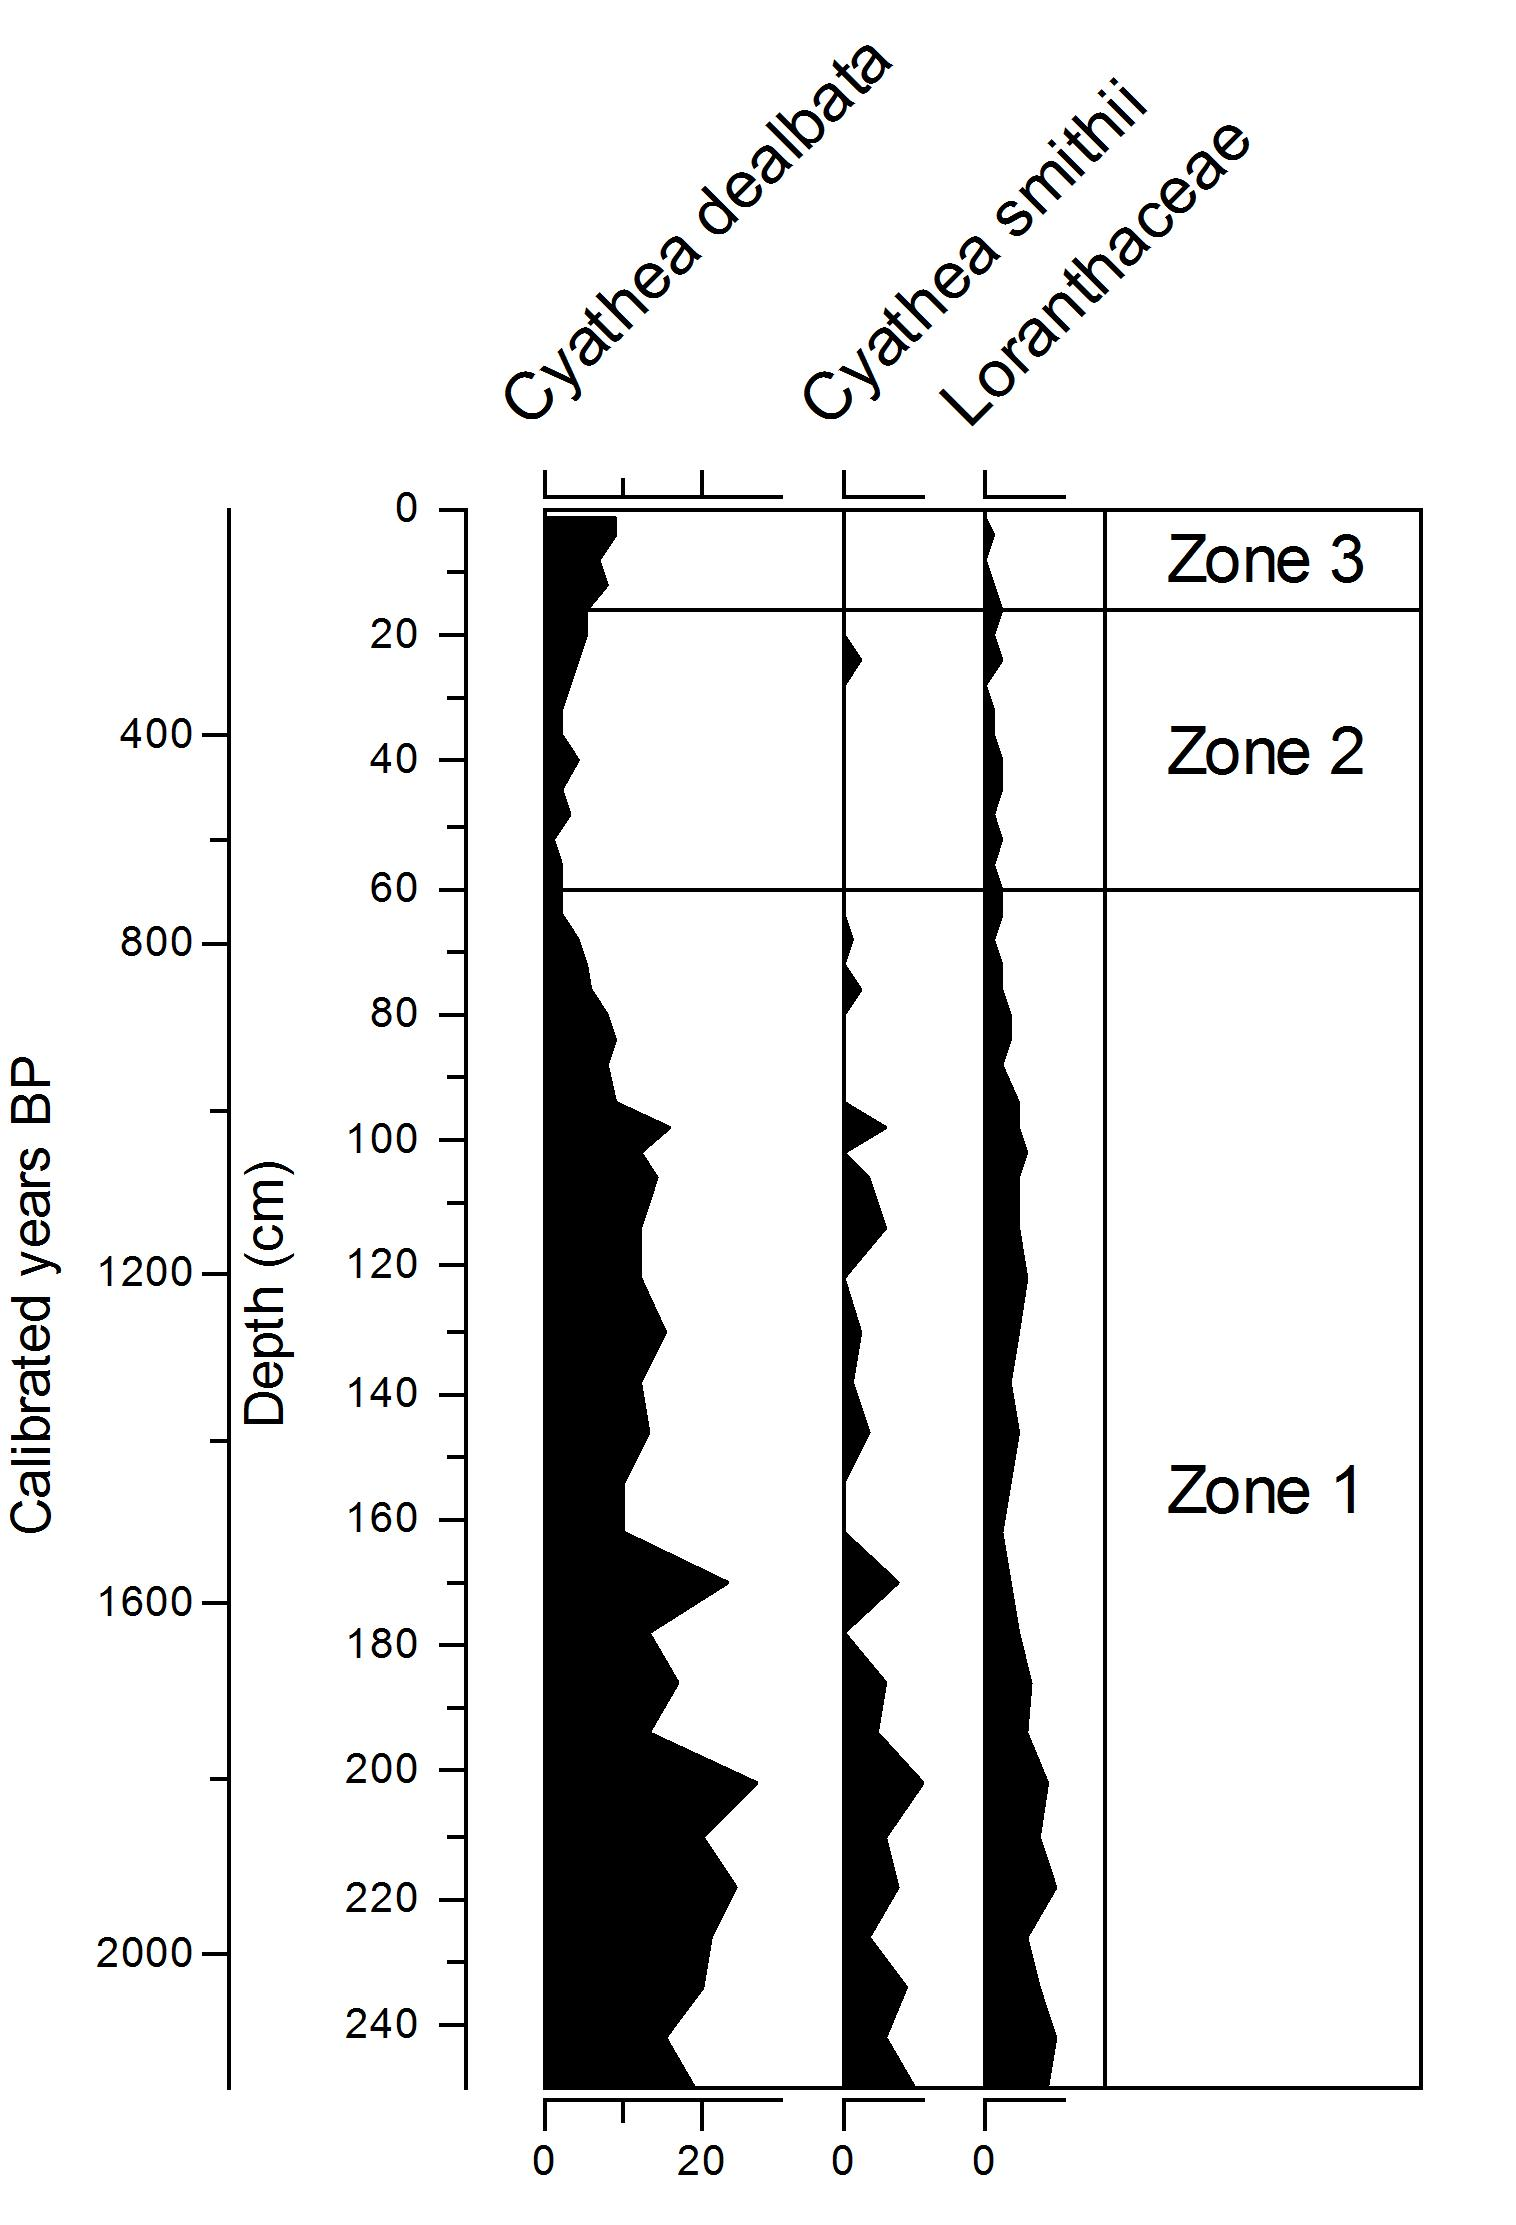
\includegraphics[scale=0.15]{ferns-zone.jpg}
	\caption[Ferns and mistletoe identified in the pollen reconstruction from Moawhitu Swamp.]{Ferns and mistletoe identified in the pollen reconstruction from Moawhitu Swamp. Pollen sum given as a percentage of total pollen count.}
	\label{fig:ferns}
\end{figure}

\subsection{Zone 2 - 150 - 650 cal. years BP}
The decline in podocarps as forest was cleared is an indication of change in zone 2 from zone 1 (Fig: \ref{fig:podo-beach-tree}, \ref{fig:disturbance}). The biggest drivers of this difference are the decrease in podocarps, and increase in grasses and bracken, as forest taxa are replaced by disturbance-tolerant species.  The creation of young and seral forest is evident in the increase in \textit{Leptospermum scoparium}  and \textit{Cordyline} pollen (Fig: \ref{fig:podo-beach-tree}, \ref{fig:disturbance}).  Large fire events during this period are evidenced by spikes in bracken, \textit{Typha} and monolete fern spores.  

\begin{figure}
	\centering
	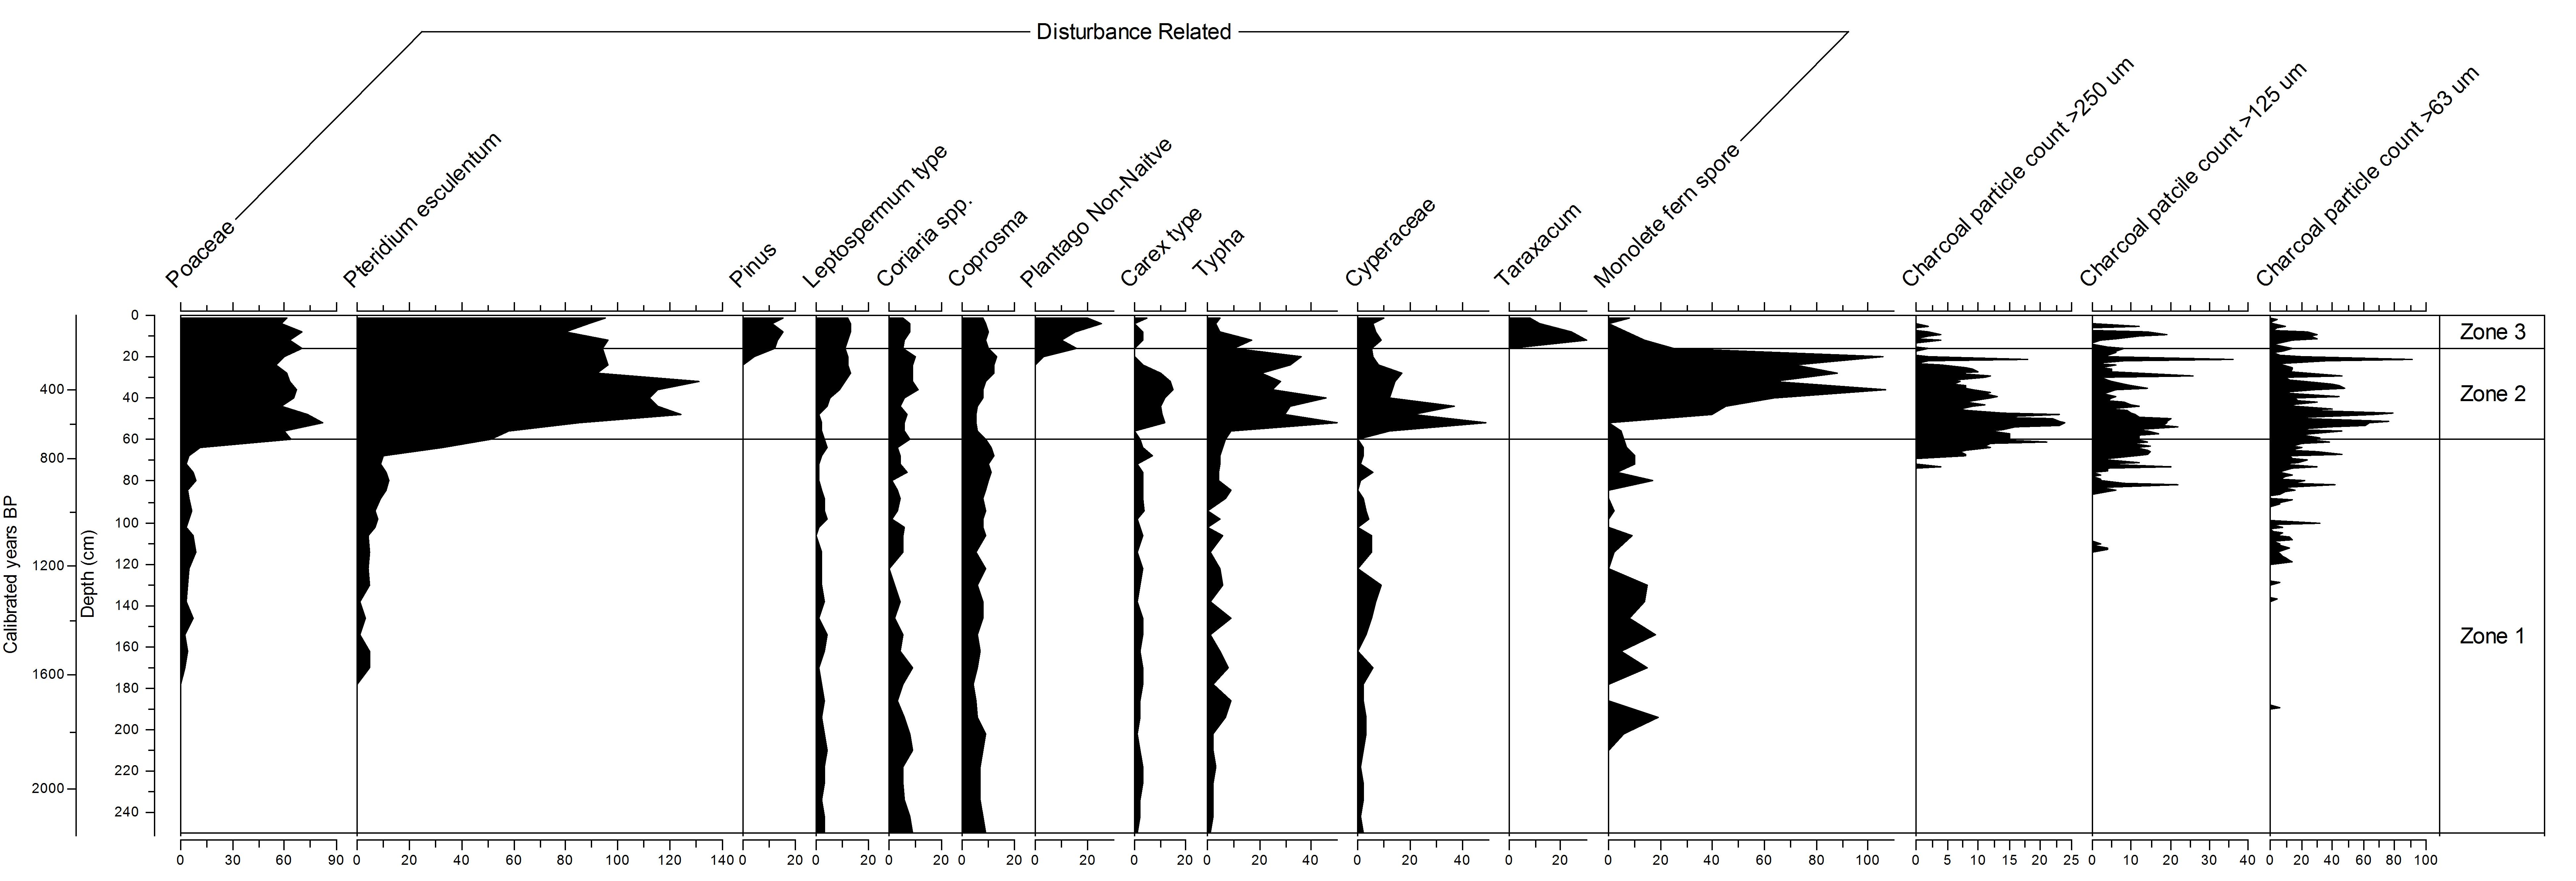
\includegraphics[scale=0.07, angle =90]{disturbance-zone.jpg}
	\caption[Changes in species associated with disturbance in pollen reconstruction from Moawhitu Swamp.]{Changes in species associated with disturbance in pollen reconstruction from Moawhitu Swamp.}
	\label{fig:disturbance}
\end{figure}

\begin{figure}
	\centering
	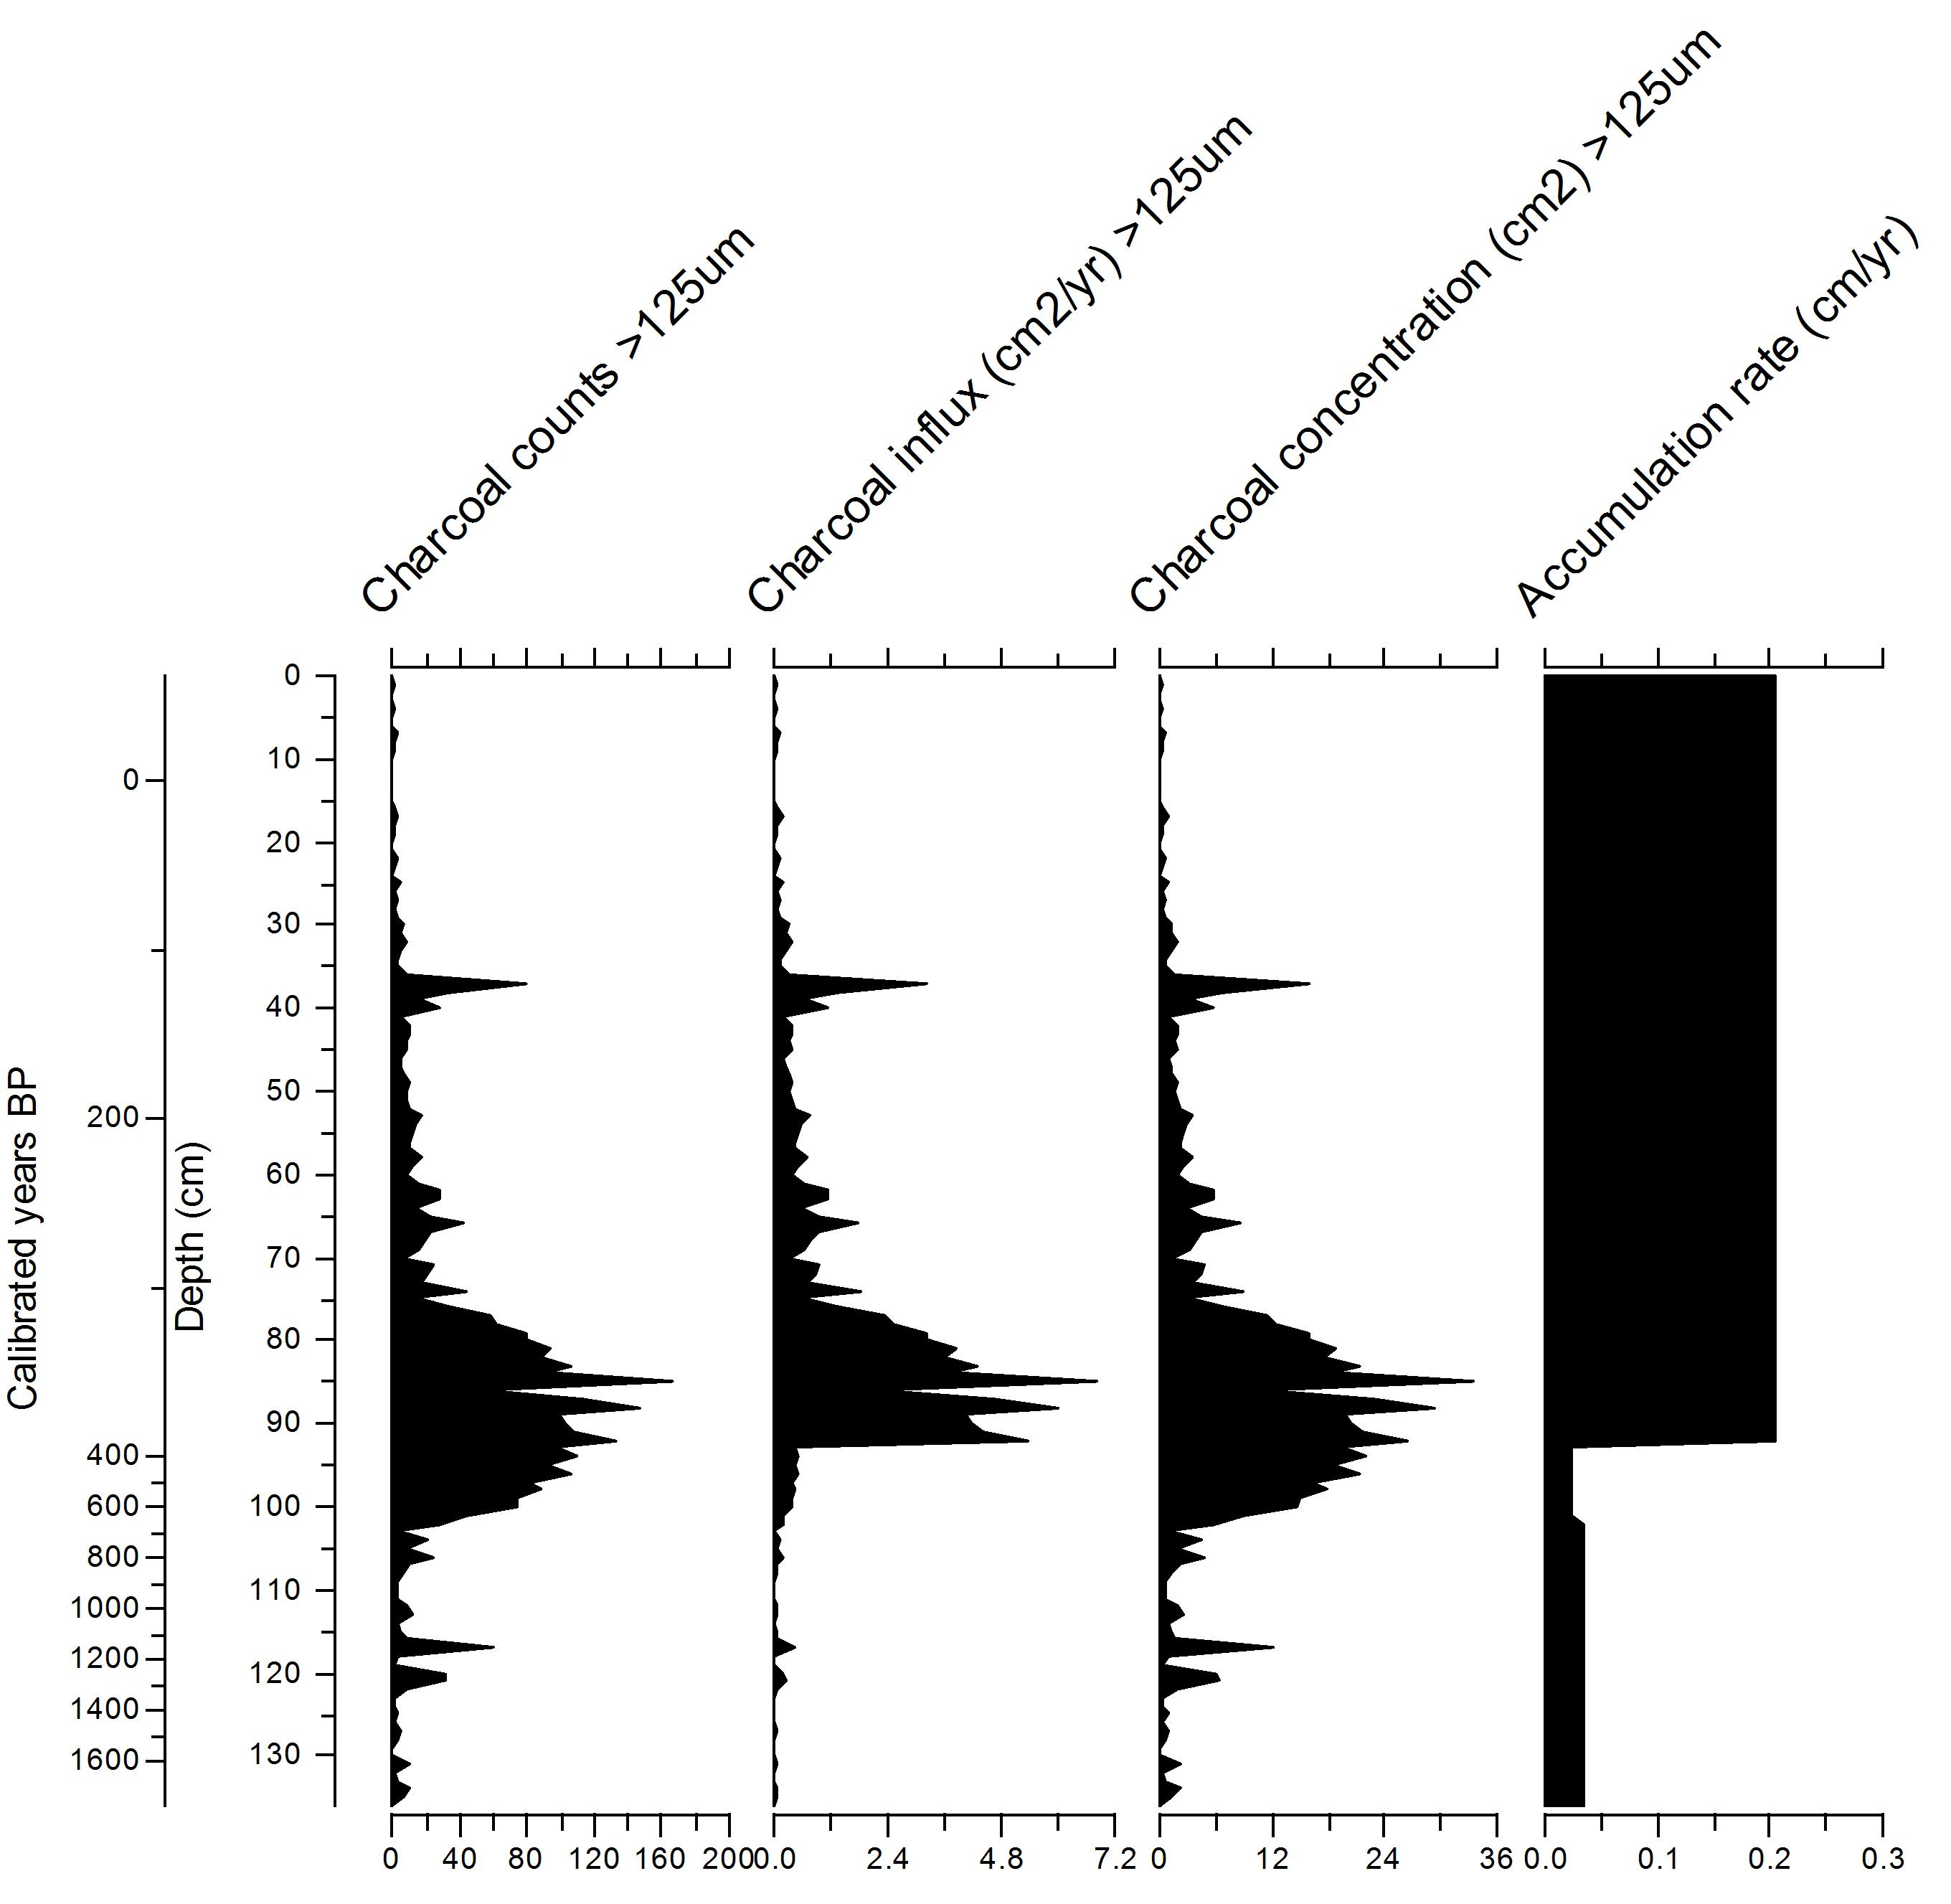
\includegraphics[scale=0.07, angle=90]{ohana.jpg}
	\caption[Changes in charcoal concentration from Ohana]{Macroscopic charcoal from the Ohana profile, expressed as concentrations and influx.  Sedimentation rates expressed as accumulation (cm/yr).}
	\label{fig:charcoal-ohana}
\end{figure}

\begin{figure}
	\centering
	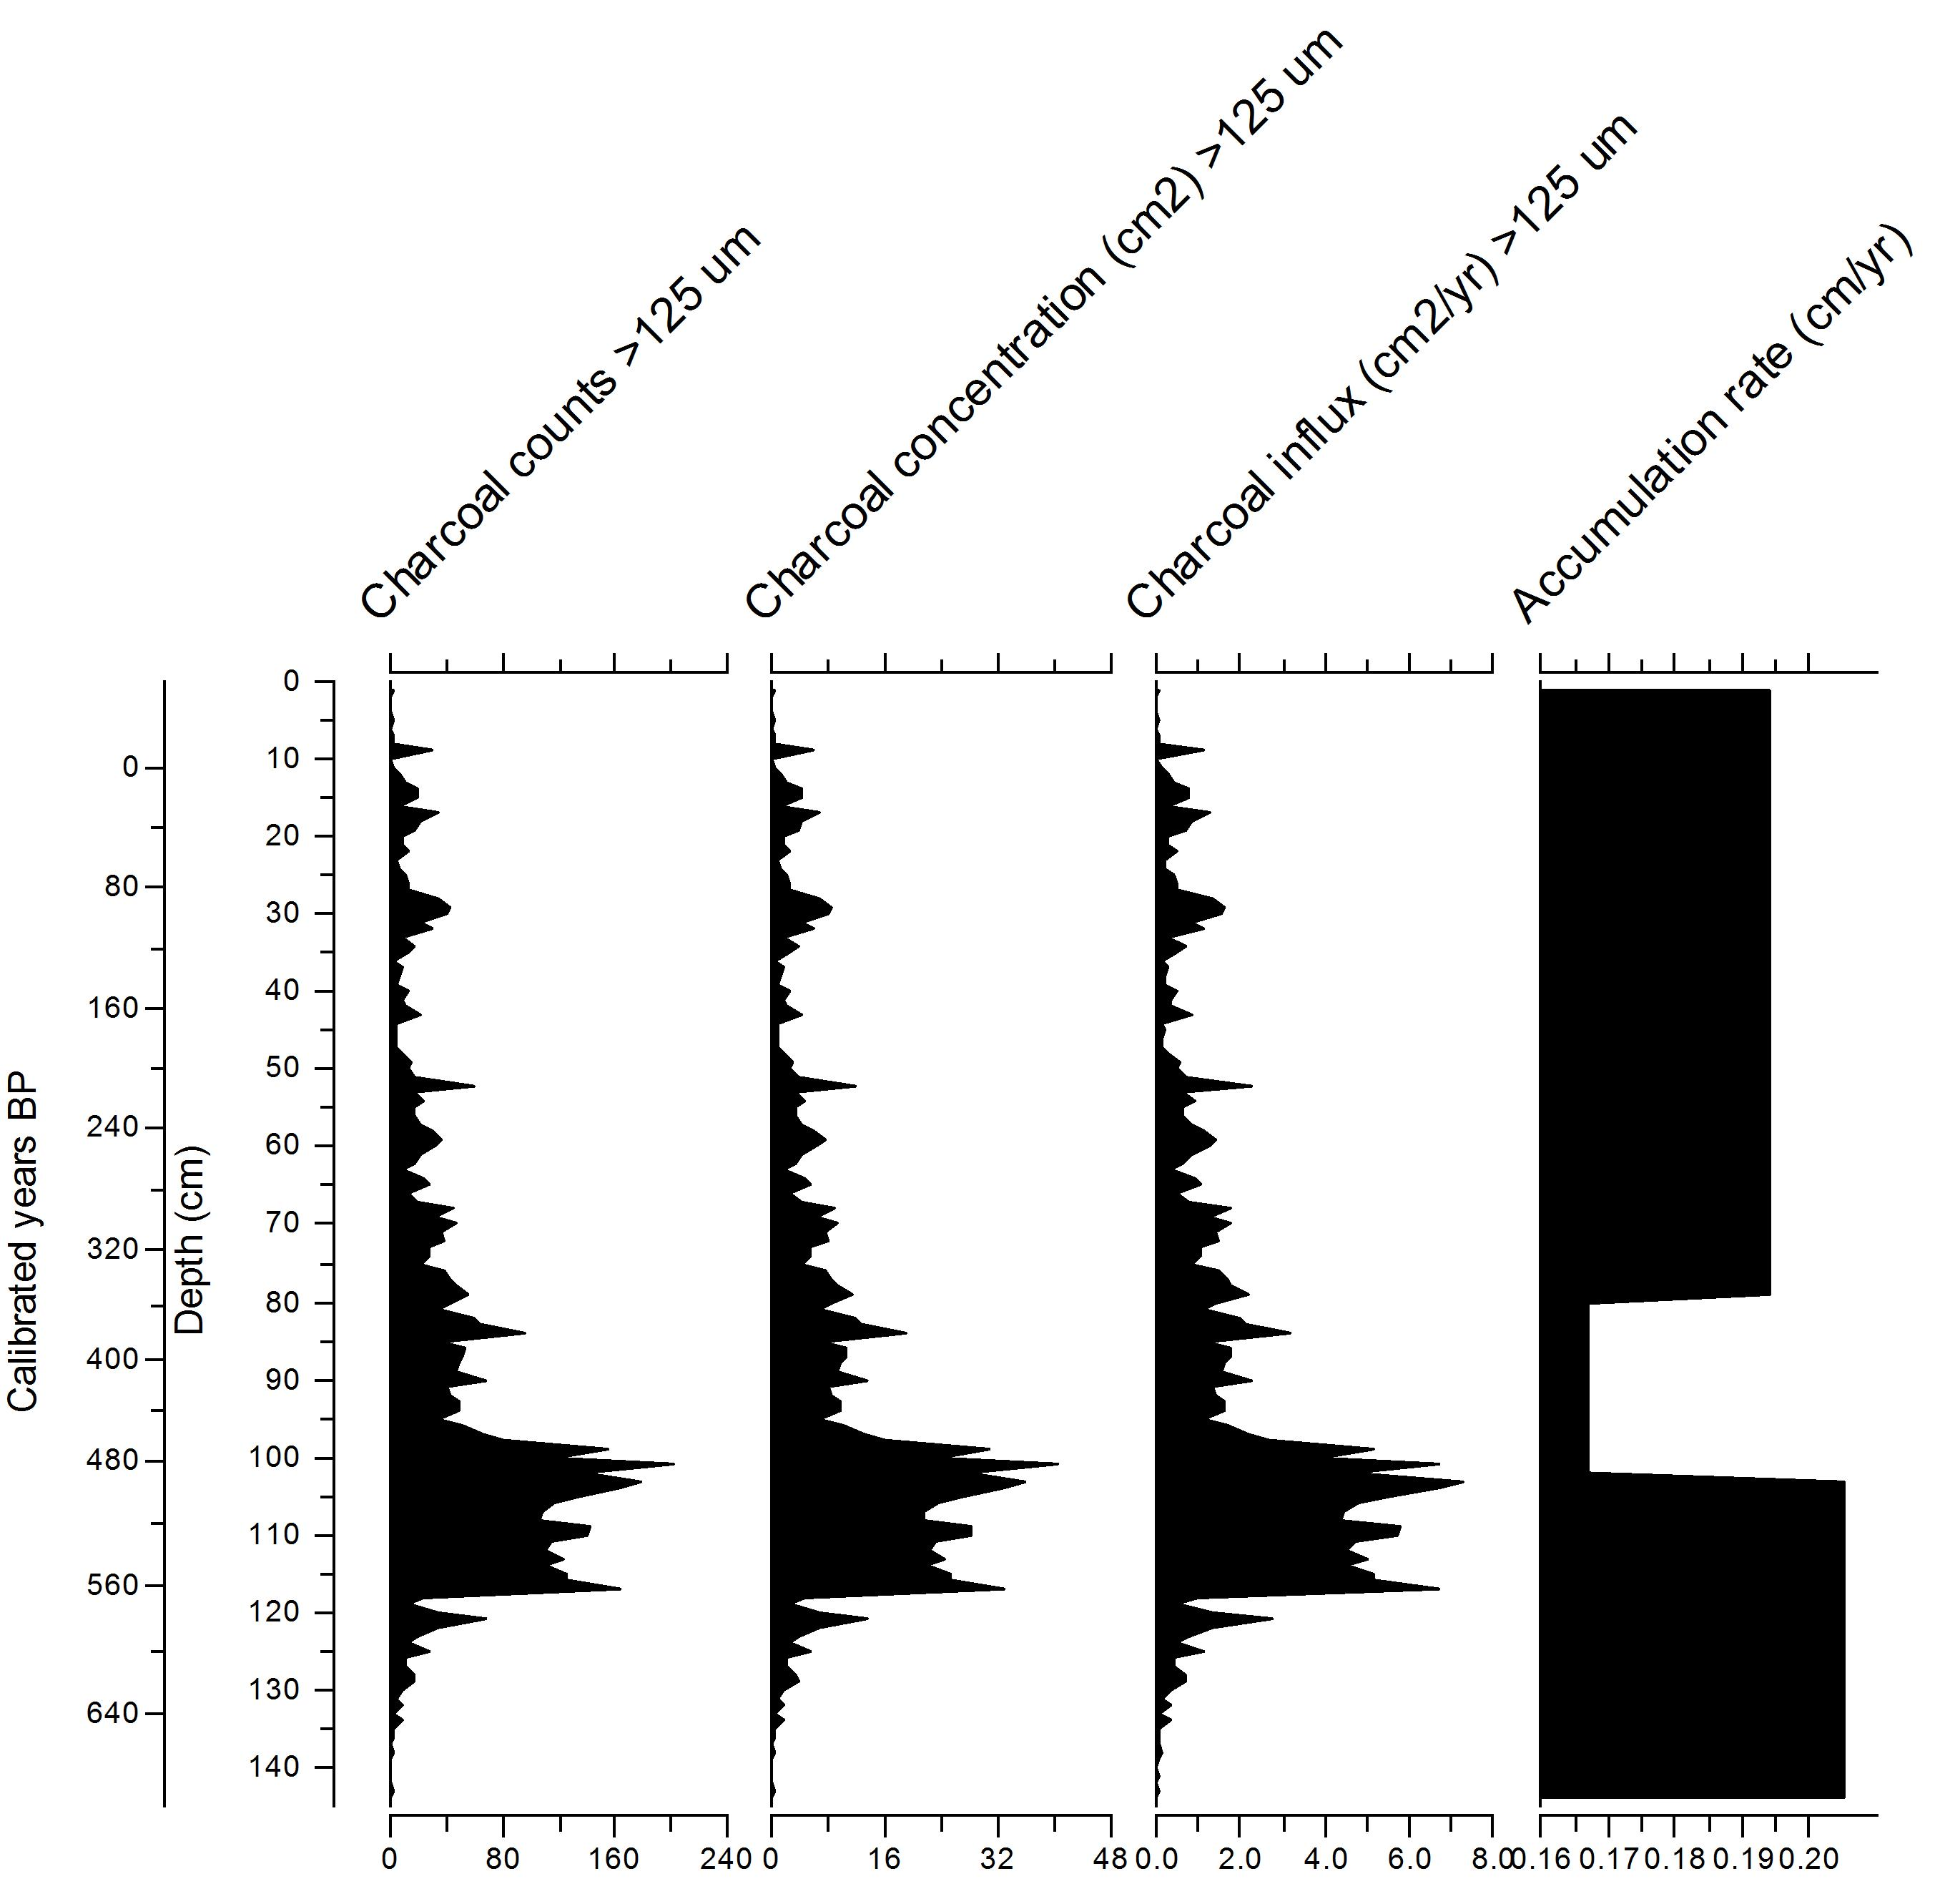
\includegraphics[scale=0.07, angle=90]{seal.jpg}
	\caption[Changes in charcoal concentration from Seal Point]{Macroscopic charcoal from the Seal Point profile, expressed as concentrations and influx.  Sedimentation rates expressed as accumulation (cm/yr).}
	\label{fig:charcoal-seal}
\end{figure}

\subsection{Zone 3 - 0 -150 cal. years BP}
The arrival or establishment of several exotic species, including \textit{Taraxacum} spp., \textit{Pinus} spp., and the non-native \textit{Plantago}, marks zone 3.  Pollen of disturbance-related taxa such as bracken, \textit{Typha} spp., and monolete fern spores contribute most to the differences observed.  Monolete fern spores and \textit{Typha} decline during this modern period and this is likely due to the reduction in fire-related disturbance events (Fig: \ref{fig:podo-beach-tree}, \ref{fig:disturbance}).  Exotics, such as \textit{Pinus} and non-native \textit{Plantago}, are also important contributors to the different vegetation communities observed.   Forest taxa, particularly podocarps, have the lowest pollen sum percentage observed across all three zones.  The open forest favours the growth of light-demanding and pioneer species such as \textit{Leptospermum scoparium}, \textit{Kunzea} spp. and \textit{Cordyline}.



\subsection{Sediment-charcoal records}

Charcoal is absent from much of zone 1 in the Moawhitu Swamp core (Fig: \ref{fig:podo-beach-tree}).  Consistent inputs of microscopic charcoal at Moawhitu Swamp begin around 1100 cal. years BP, with three peaks at c. 490, 470 and 228 cal. years BP. All three sites show increasing macroscopic charcoal inputs from around 650 cal. years BP onwards, with charcoal concentrations being highest from  400 - 600 cal. years BP (Fig: \ref{fig:podo-beach-tree}, \ref{fig:charcoal-ohana}, \ref{fig:charcoal-seal}).  The Ohana Lake profile also exhibits another charcoal peak at 120 cal. years BP after a steady decline, with Seal Point also showing higher concentrations around this period (Fig: \ref{fig:charcoal-ohana}, \ref{fig:charcoal-seal}).  The Moawhitu Swamp core is more temporally variable in terms of charcoal concentration, but shows a similar pattern of increased burning at around 100 cal. years BP (Fig: \ref{fig:podo-beach-tree}).  A visual comparison of charcoal concentration and influx from the Moawhitu and Seal Point cores reveals close agreement in temporal pattern across size classes (Fig: \ref{fig:podo-beach-tree}, \ref{fig:charcoal-seal}).  A dramatic increase in accumulation after nearly three centuries of increased charcoal inputs correlates with increases in charcoal influx just after 400 cal. years BP in the Ohana core (Fig: \ref{fig:charcoal-ohana}).    


\subsection{Magnetic susceptibility} 

Corresponding with Polynesian arrival, magnetic susceptibility increases  from c. 600 cal. years BP in the Seal Point core. This rise in magnetic susceptibility peaks c. 175 years later, and then shows a fluctuating decline until European arrival (c. 150 cal. year BP), when magnetic susceptibility increases until a peak c. 120 cal. years BP, gradually declining thereafter.  Polynesian settlement does not give a clear signal in the Ohana core, with magnetic susceptibility declining c. 600 cal. years BP. This decline continues for c. 200 years before we see increases to the highest magnetic susceptibility levels seen in the core. European settlement provides a clearer signal in the Ohana core, with similar magnetic susceptibility increases c. 150 cal. years BP to those in Seal Point.  Charcoal and magnetic susceptibility were not significantly correlated in either the Seal Point or Ohana profiles, (r=0.179 and r=0.157, respectively), however there is a significant lagged correlation between fire activity (as measured by charcoal) and magnetic susceptibility. The maximum correlation occurs when a lag of 22 cm is applied (r=0.541, P <0.05) or approximately 60 years to the Seal Point core.  Correlation also improves (r=0.547, P <0.05) when a 50 year lag is applied to the Ohana profile.       


\begin{figure}[H]
	\centering
	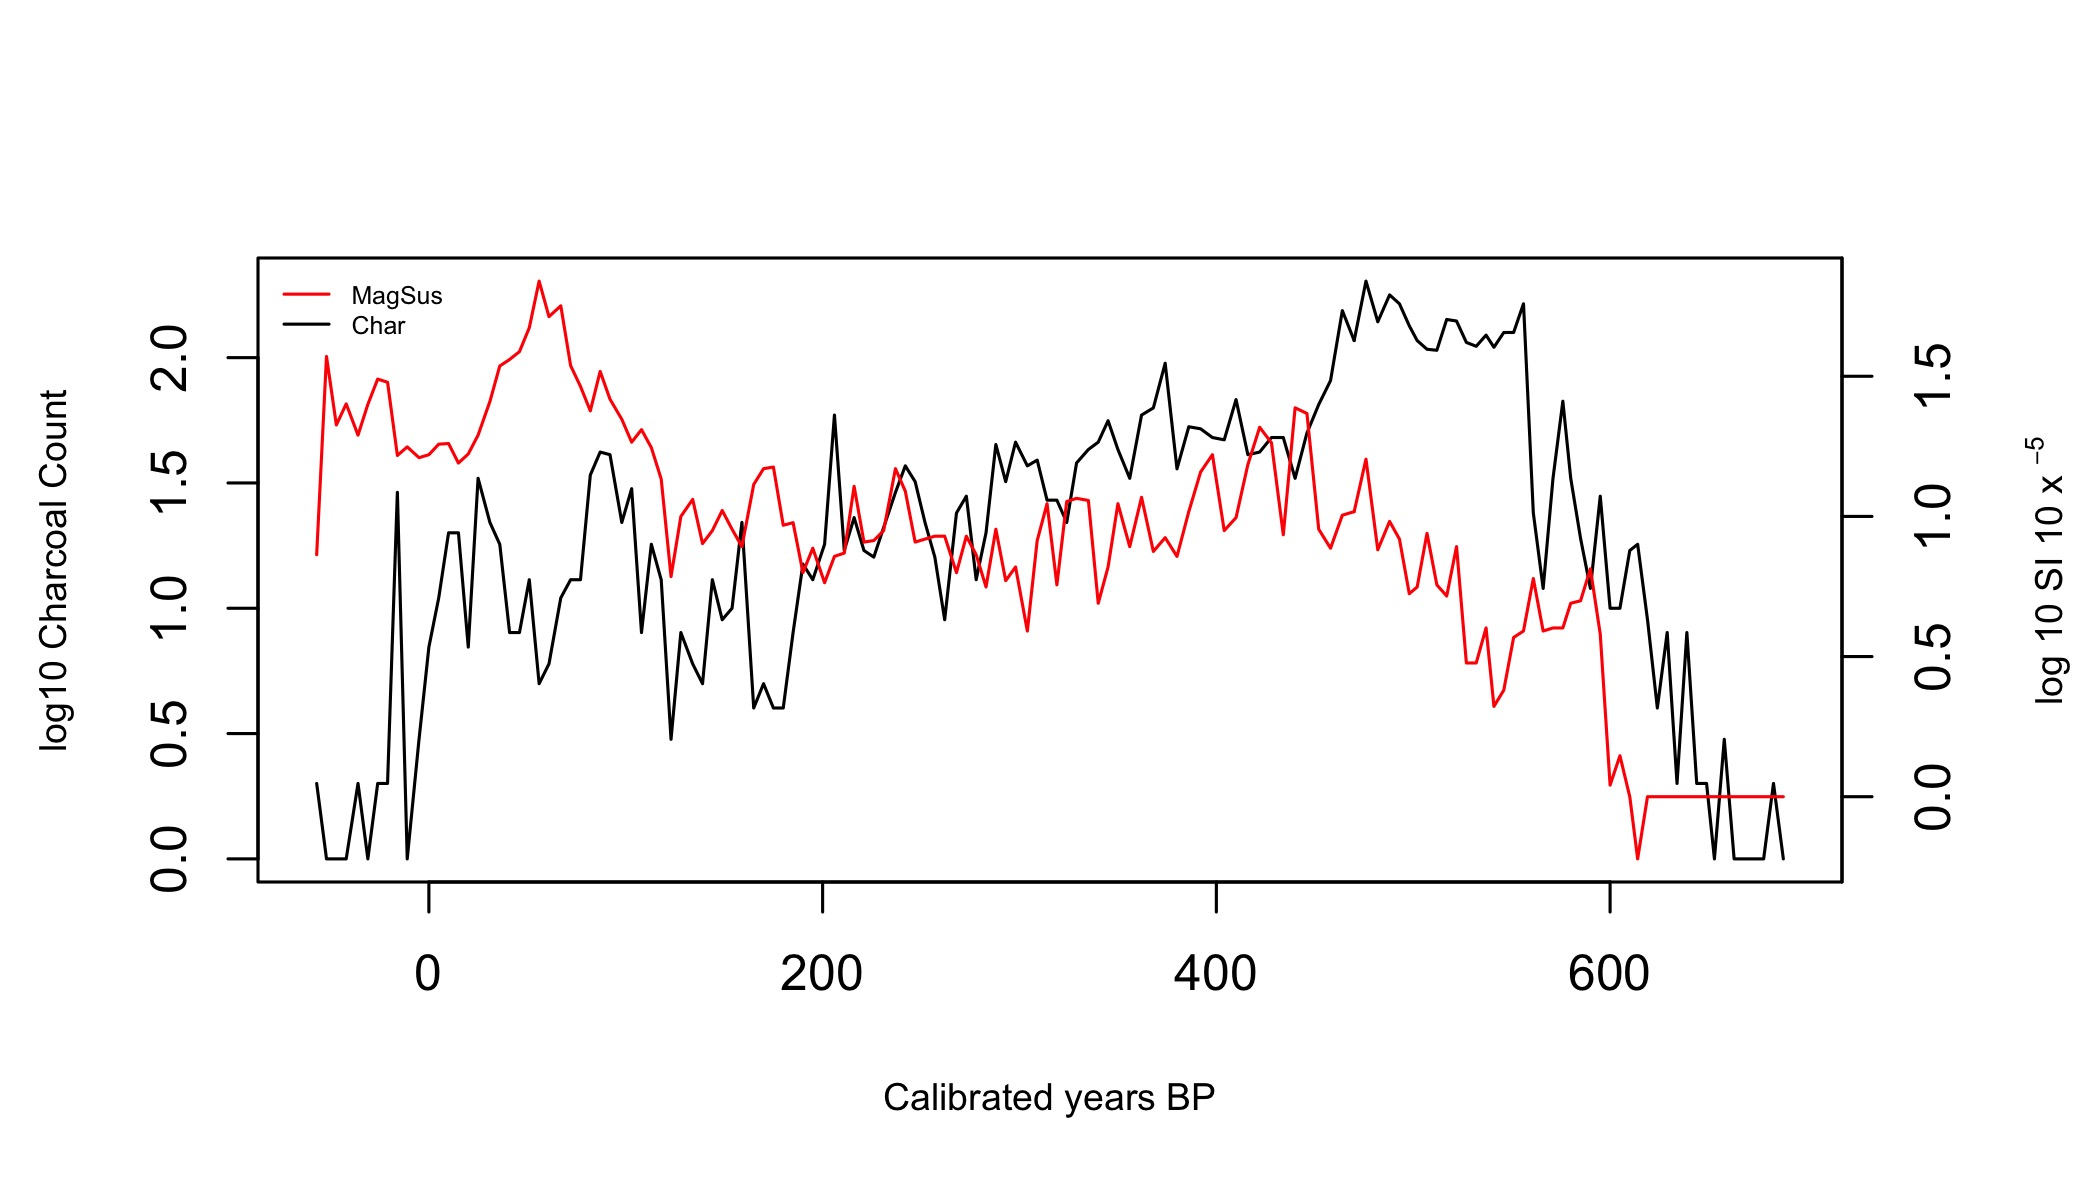
\includegraphics[scale=0.2]{mag-sus-seal.jpeg}
	\caption[Magnetic susceptibility (log10) and charcoal particle count (log10) from the Seal Point core]{Magnetic susceptibility (log10) and charcoal particle count (log10) from the Seal Point core.}
	\label{fig:mag-sus-seal}
\end{figure}

\begin{figure}[!ht]
	\centering
	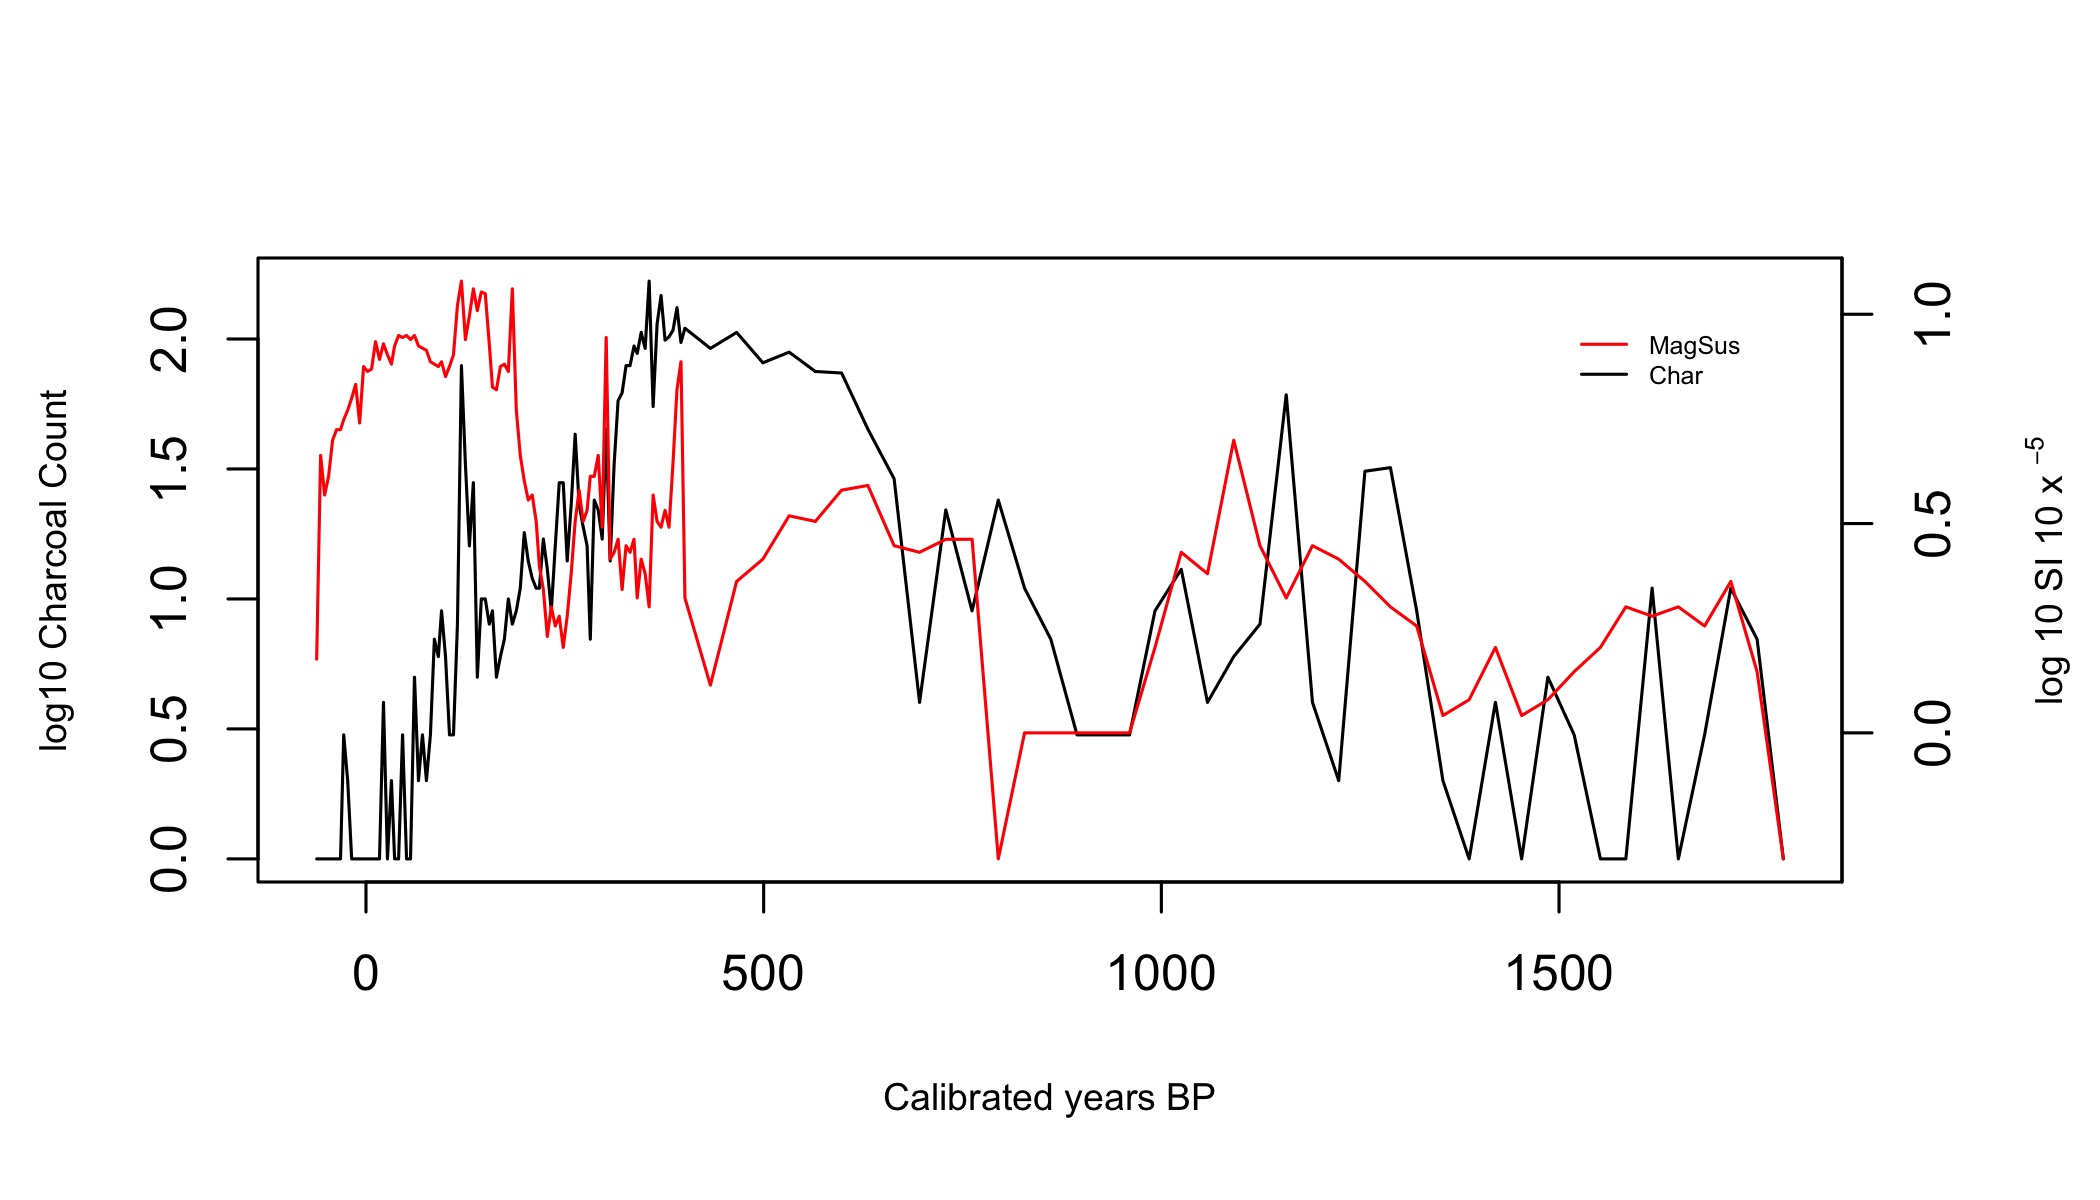
\includegraphics[scale=0.2]{mag-sus-ohana.jpeg}
	\caption[Magnetic susceptibility (log10) and charcoal particle count (log10) from the Ohana core]{Magnetic susceptibility (log10) and charcoal particle count (log10) from the Ohana core.}
	\label{fig:mag-sus-ohana}
\end{figure}

\subsection{Definition of settlement and prehuman zones using all
proxies}

Previous work by \cite{Wilmshurst2008} places Polynesian settlement of New Zealand at c. 1280 AD. Based on the combination of sustained burning, decline of forest (Fig: \ref{fig:podo-beach-tree}) and increase in disturbance related taxa in the pollen record (Fig: \ref{fig:disturbance}), settlement of D'Urville Island likely began c. 650 cal years BP, corresponding to a depth of c. 64 cm in the Moawhitu Swamp core (Fig: \ref{fig:disturbance}).  This Polynesian settlement period represents zone 2 in the ordination presented (Fig:\ref{fig:ordination}), and shall be referred to as such hereafter; zone 1 will be identified as prehuman (Table:  \ref{t:zone-name}).

Exotic pollen taxa are a clear signal of European settlement and so their arrival c. 150 cal. years BP make the European zone easier to identify. \textit{Pinus}, non-native \textit{Plantago} and \textit{Taraxacum} appear at 20 cm in the Moawhitu Swamp core.  Unfortunately, the lack of radiocarbon dates towards the top of all three cores, combined with the notorious difficulty in dating periods ranging from 1800 to 1950 AD \citep{hajdas2008radiocarbon} (a result of increases in fossil fuel combustion during the industrial revolution), creates a high degree of uncertainty in this zone. However, reliable records show permanent European settlement of D'Urville Island followed that of other New Zealand locations in 1840 AD, with the arrival of the first immigration ships at Port Hardy (a large inlet to the north of  D'Urville Island) \citep{walls}.  Given these historical dates for European arrival, and the appearance of exotic taxa in the pollen reconstruction, it is safe to assume that European arrival occurred at around 20 cm (c. 150 cal. years BP), encompassing zone 3 (Fig: \ref{fig:ordination}). The relevant depths, mean cal. years BP, zone numbers and subsequent names are given in Table \ref{t:zone-name}.    

\begin{table}[H]
	\caption{Zones identified as a result of age-depth model, pollen and charcoal analysis from all three cores.}
	\centering
	\label{t:zone-name}
	\begin{tabular}{c c c c }
		\noalign{\smallskip} \hline \hline \noalign{\smallskip}
		Depth (cm) & Mean estimate of cal. years BP & Zone Number & Zone Name  \\ \hline
		                             0 - 20 cm                               & 0 - 150                        & 3           & European   \\
		                             20 - 64 cm                              & 150 - 650                      & 2           & Polynesian \\
		                            64 - 250 cm                              & 650 - 2120                     & 1           & Prehuman   \\
		          \noalign{\smallskip} \hline \noalign{\smallskip}           &
	\end{tabular}
\end{table}

%------------------------------------------------

\section{Discussion}

Analysis of the data from the three sites considered in this study provide a first look at the late Holocence vegetation and fire history of D'Urville Island in the Marlborough Sounds, New Zealand. Pollen assemblages, macroscopic and microscopic charcoal in the sediment profile from Moawhitu Swamp provide a 2200 year record of vegetation shifts and fire history.  Cores taken from Seal Point and Ohana Lake date back to c. 688 and c. 1782 cal. years BP, respectively. This study confirms that fire was a rare event prior to human arrival on the island, but c. 650 cal. year BP, and coincident with human arrival, it dramatically increased.  The introduction of exotic plant species following European arrival c. 150 cal. year BP further complicates an already highly altered ecosystem.

\subsection{What were the pre-human plant assemblages?}

The lack of change in pollen percentages during the pre-human zone suggests relatively stable vegetation assemblages (Fig: \ref{fig:podo-beach-tree}). It is unlikely that large disturbance events on D'Urville Island occurred with any frequency prior to human settlement, although it has been suggested that a tsunami struck the island around the 16\textsuperscript{th} century \citep{mitchell2007history}; however, there is no evidence in the pollen reconstruction for such an event.  We see a clear and persistent dominance of Nothofagaceae  throughout the pre-human period, on average accounting for over 50\% of the total pollen sum (Fig: \ref{fig:podo-beach-tree}). During this pre-human period Nothofagaceae forest is associated with a tall emergent layer of podocarp species including \textit{Dacrydium cupressinum}, \textit{Dacrycarpus dacrydioides}, \textit{Prumnopitys ferruginea}, \textit{Prumnopitys taxifolia} and \textit{Podocarpus totara}.  This Nothofagaceae-\textit{Podocarpus} forest would have been accompanied by a diverse canopy of \textit{Weinmannia} spp., \textit{Nestegis} spp. and \textit{Elaeocarpus} spp.  Smaller trees in the sub-canopy include \textit{Coprosma} spp., \textit{Alectryon excelsus} and \textit{Dodonaea viscosa}.  Climbers such as \textit{Rubus} spp. also occur in the pollen record.  Shrubs associated with forest margins including \textit{Aristotelia} spp., \textit{Melicytus} spp., \textit{Pseudopanax} spp., \textit{Myrsine } spp., \textit{Coprosma} spp., \textit{Rubus} spp., and bracken are consistent throughout.  \textit{Dysoxylum spectabile}, \textit{Aristotelia serrata}, \textit{Rhopalostylis sapida} and \textit{Leptospermum scoparium} would have been abundant, likely on coastal slopes and gullies. Tree-ferns, namely \textit{Cyathea dealbata} and \textit{Cyathea smithii}, would have been present in both gully forest and the understory (Fig: \ref{fig:ferns}).  Low forest climax vegetation such as \textit{Pseudopanax} spp, \textit{Metrosideros} spp. and \textit{Dacrycarpus dacrydioides} would have been far more prominent and likely not restricted to the higher elevations they are today.  Rich palm and \textit{Dysoxylum} forest would have surrounded the lakes, wetlands and coastal areas.  

Mistletoe are abundant throughout the pre-human phase, and although only identified to the family level, the species are likely \textit{Alepis flavida}, \textit{Peraxilla colensoi} and \textit{Peraxilla tetrapetala} given their association with beech \citep{norton1999host}.  The historic abundance of mistletoes (up to 8\% of total pollen sum, Fig: \ref{fig:ferns}) can offer important baseline guidelines for restoration, given their current threatened conservation status \citep{sweetapple2002mistletoe}.    

\subsection{Pollen record after Polynesian settlement}

The rise in sediment charcoal, combined with shifts in pollen taxa, clearly indicates human arrival at c. 650 cal years BP. Settlement brought increased fire frequencies on D'Urville Island, and with this there is a clear shift in both the dominant species and the nature of the plant assemblages.  A common characteristic among the species that follow periods of increased fire activity is they are favoured in post-fire environments.  The evidence provided here certainly follows that pattern, with bracken and grass abundance dramatically increasing, and subsequently persisting in the pollen reconstruction.  Disturbance-related species also drive much of the differences observed between the pre-human and Polynesian zones (Fig: \ref*{fig:disturbance}). \textit{Typha} also increases substantially and comprises up to 15\% of the pollen sum in some years (Fig: \ref{fig:disturbance}).  This increase, in what is a nutrient-loving species, likely reflects an influx of detritus, sand and silt into both lake and swamp areas as a result of increased burning, and is a common response following deforestation in New Zealand wetlands \citep{McGlone1999}.  An increase in sediment accumulation rates from Ohana support this hypothesis (Fig: \ref{fig:charcoal-ohana}). \textit{Typha} pollen was also used by Maori to make cakes, with the roots providing a food source \citep{taylor2010te}, and deliberate action to support this practise could have contributed to its expansion.  Magnetic susceptibility also increases during this period suggesting inputs from erosion as a result of the loss of forest cover (Fig: \ref{fig:mag-sus-seal}, \ref{fig:mag-sus-ohana}).    
	
\subsection{Pollen record after European settlement}

Forest taxa show little  recovery during the European period, although beech does increase to around 15\% of the pollen sum (Fig: \ref{fig:podo-beach-tree}).  Beech is known to colonise small disturbed areas rapidly; however, its heavy seeds mean that it can be dispersal limited, recovering slowly without adequate seed sources \citep{Wardle1984}. On D'Urville Island this process is likely hampered by the rise of fire-adapted species such as \textit{Leptospermum scoparium}, \textit{Kunzea} spp., \textit{Pinus} spp. and \textit{Cordyline} spp.  The emergence of \textit{Pinus} in the pollen record is a familiar signal of European arrival. Pasture plants such as \textit{Trifolium} spp. and exotic members of the Poaceae also appear. Pines were introduced to NZ early in the 20\textsuperscript{th} century, and can be seen invading serpentine (ultramafic) areas on D'Urville. Bracken and grasses, limited before the introduction of fire, dominate the pollen record (Fig: \ref{fig:disturbance}) and we see the arrival of other non-native taxa, including \textit{Taraxacum} and \textit{Plantago}. 

\subsection{The charcoal record}

The microscopic and macroscopic charcoal records reveal that fire was not a regular occurrence on D'Urville Island or the surrounding area until c. 650 cal. years BP. The macroscopic charcoal record shows a similar pattern, and, given the larger particle size, provides a better understanding of localised fire \citep{leys2013}.  The long absence of fire in this record is not surprising given: a) the relatively short period examined, and b) the evidence that fire events were often centuries apart in pre-human New Zealand \citep{OgdenJ,McGlone1998,McGlone1999,Wardle2001}.  Interestingly there are some macroscopic peaks between 1288 and 1256 cal. years BP, and another at c. 1157 cal. years BP in the Ohana core (pre-human zone).  In the Moawhitu Swamp core these peaks are just discernible in the microscopic charcoal record.  These peaks are likely the result of small wetland fires, common in these environments and unlikely to have impacted the surrounding forest, a dynamic observed in wetland fires elsewhere \citep{mcglone1984vegetation}.  The magnetic susceptibility signal also supports the presence of fire in the pre-human zone as we see a clear spike during this period (1288 and 1256 cal. years BP) (Fig: \ref{fig:mag-sus-ohana}).  Pollen reconstruction from Ohana would allow further investigation of these fire events. 

The \textquotesingle {Initial Burning Period\textquotesingle} (IBP) in the decades immediately after Polynesian settlement (c. 1280 AD) was responsible for transforming large parts of the South Island's native forests  \citep{McWethy2009a}, and was likely facilitated by positive feedbacks between fire and vegetation \citep{perry2015exotic}.   Given the limited amount of charcoal prior to this period, no evidence for dramatic climatic shifts \citep{McWethy2009a}, we can assume the input of charcoal comes from anthropogenic fire on D'Urville Island, and follows a similar pattern of deliberate  and systematic fires to those in other locations during the IBP.  Fire was also an important part of Maori culture, used to remove scrub and forest\citep{grace2015}.  This process of burning also not only deprived wild game of cover, it aided in the growth of understory shrubs, particularly bracken, an important food source \citep{guild2009history,Wilmshurst2005}.  Fire also enabled the first settlers to clear land quickly for horticulture, and the cultivation of crops including k\=umara (\textit{Ipomoea batatas}) \citep{simmons1969economic}.           

Inferences beyond the timing of fires on D'Urville Island, as with any interpretation of paleo-charcoal, present challenges.  Although we can be confident that fire most certainly occurred in the region from 650 cal. years BP, it is difficult to determine the spatial patterns of this activity.  It is likely that human populations were concentrated around argillite quarries \citep{walter2010colonisation}.  Burning would likely have commenced in the low land areas with easy access to water that were most suitable for settlement and horticulture.  This is the pattern described in \cite{Perry2012} for New Zealand as a whole.  The higher elevation areas would probably have been cleared later or accidentally burnt.  The episodic nature of the charcoal records suggests temporal variation in fire events corresponding to anthropogenic activity; indeed, the small quantities of macroscopic charcoal earlier in the record indicates that the introduction of regular fire was rapid.  Increases in charcoal deposition also correlate with increases in disturbance-related pollen taxa (Fig: \ref{fig:disturbance}) and the loss of forest taxa (Fig: \ref{fig:podo-beach-tree}).  These factors, combined with D'Urville Island's distance from the mainland (0.6 km), provide confidence  that the macroscopic charcoal record demonstrates the onset of relatively large localised fires.  It is important to acknowledge previous work that suggests macroscopic charcoal can travel several kilometres from its source during wildfires \citep{tinner1998,Tinner2006}.  Hence, there is the potential that macroscopic charcoal particles could come from locations outside of D'Urville, but this is unlikely given the abundances seen.  

Given the loss of closed canopy forest indicated in the pollen record (Fig: \ref{fig:podo-beach-tree}), it is likely that these post-settlement fire events were consistent re-burns of early successional vegetation rather than in previously unburned areas \citep{Perry2014}.  The loss of woody material after the IBP would explain the decrease in macroscopic charcoal inputs, until a small spike occurred during the European period (Fig: \ref{fig:disturbance}, \ref{fig:charcoal-ohana}, \ref{fig:charcoal-seal}).  It is also likely that Polynesian interests in the islands were diminishing given intensive warfare and decreasing trade in argillite \citep{Wellman1962}.  European settlement did not signal a respite for D'Urville Island, and the charcoal record demonstrates a continuation of burning, albeit somewhat subdued.  The decrease in charcoal deposits are, in part, likely due to the adoption of different land clearing methods by European settlers (e.g. physical removal of scrub) and a decrease in fire-related land clearance methods. Despite the reduction in charcoal input, it appears that the beech-podocarp and coastal rich palm forest did not recover after the IBP, and that fire and land management practises continue to be a significant disturbance mechanism.

\subsection{Magnetic susceptibility}

Soil magnetic susceptibility increases with the onset of the IBP but shows a consistent decline thereafter (Fig \ref{fig:mag-sus-seal}, \ref{fig:mag-sus-ohana}).  This trend is more prominent in the Seal Point record; although we do see an increase in magnetic susceptibility at Ohana, it is less pronounced until some time after the IBP.  Charcoal and magnetic susceptibility do not correlate well in either the Seal Point or Ohana records (r=0.179 and r=0.157, respectively, Fig: \ref{fig:mag-sus-seal}, \ref{fig:mag-sus-ohana}).  Interestingly we see the lowest correlations after Polynesian settlement and during the IBP (c. 550 - 420 cal. years BP), and after European settlement (c. 150 cal. years BP) (\ref{fig:mag-sus-ohana}).  This lack of correlation indicates that an increase in charcoal deposits is not synchronous with changes in magnetic susceptibility.  This pattern is supported by strengthened correlation in both Seal Point and Ohana (r=0.541 and r=0.547, respectively) when approximately 40-60 year time lags are applied to magnetic susceptibility, implying that changes in magnetic susceptibility are, at least in part, likely due to erosion events rather than magnetic enhancement of soils as a result of burning (i.e. the gradual degradation of forest slowly reducing soil cohesion and subsequently increasing input of allochthonous mineral material from erosion). Erosion is certainly well correlated with deforestation in New Zealand, with \cite{wilmshurst1997impact} noting significant erosion pulses in lake sediment cores as a result of deforestation during settlement in Lake Tutira, Hawke's Bay area, North Island, New Zealand. \cite{McWethy2009a} showed magnetic susceptibility was almost simultaneous with the onset of burning in some sites examined in the South Island, New Zealand, and its decline strongly associated with the end of the IBP. They suggest watershed vegetation was highly impacted, resulting in erosion events almost immediately after fire. 

We suggest that the time-lags observed in correlations between charcoal and magnetic susceptibility at D'Urville Island are, at least in part, due to a once abundant beech-podocarp forest being slowly degraded, with the associated deposition of allochthonous mineral increasing gradually over time rather than abruptly.  The strengthened correlation after the IBP with a lag applied supports this hypothesis, suggesting that the process of burning removed riparian vegetation, and thus deposition rates increased.  It can be argued that the gradual decline in magnetic susceptibility towards the end of the Polynesian and beginning of the European zone is due to the increased cover of bracken, known to stabilise soils after deforestation \citep{wilmshurst1997impact,Wilmshurst2005}.  The stabilisation afforded by bracken is potentially site-specific, and hence we witness different patterns in accumulation rates between Ohana and Seal Point (Fig: \ref{fig:charcoal-ohana}, \ref{fig:charcoal-seal}).
      

\subsection{The consequences of human settlement}
The removal of large quantities of forest, and the decline in species-rich palm and \textit{Dysoxylum} forest leaves parts of D'Urville Island vulnerable to further disturbance events, and ongoing invasion by the exotic species already established.  The dominance of bracken and Poaceae in the pollen record, combined with the expansion of \textit{Leptospermum} spp. and \textit{Pinus} spp. is symbolic of a landscape that has been highly disturbed. Such sites can quickly become fire-prone amplifying a `fire begets fire' feedback dynamic.  Colonisation by later successional species is made increasingly difficult by the already limited remnant forest and respective seed sources remaining on D'Urville Island.  This  positive feedback is suggested by \cite{Perry2014}; the post-vegetation landscape is more flammable, making the system more susceptible to fire, and hence harder for later succession species to establish.  Gorse (\textit {Ulex europaeus}), although not present in the pollen record but prevalent on D'Urville Island, will contribute to the fire-prone nature of early successional locations given the high ignitability of its litter \citep{madrigal2012evaluation}; it was the most flammable, at the shoot-level, of the 60 species assessed by \cite{wyse2016quantitative}.   Further disturbance events, be they fire or other natural occurrences such as drought, will result in the colonisation of species well-adapted to disturbed environments.  Feedbacks between disturbance and invasive plant taxa can potentially result in broad areas of homogeneous early successional vegetation that reduce the potential of native flora to establish \citep{gaertner2014invasive}. 

The \textquotesingle{fire begets fire\textquotesingle} pattern is shown by the transition from an old landscape, dominated by the species prominent in the pre-human period, to a young, fire prone system comprised of other species that established in the late Polynesian/early European period on D'Urville Island.  Although fire activity has certainly decreased in recent years, the dominant vegetation that remains will be highly susceptible to natural, or accidental fire events.  Seedling establishment in these early-successional environments is likely further hampered by browsing from rats (\textit{Rattus rattus}) present on D'Urville Island \citep{wilson2003effects}.  Breaking this cycle is extremely difficult as the system could be characterised as having shifted to an alternative stable state reinforced by strong positive feedbacks \citep{bowman2015feedbacks}.  These systems then exhibit a difficult to reverse shift in both vegetation structure and composition \citep{Perry2014}. Such multi-stressed environments increase the complications for restoration as a result of non-independent pressures, requiring each stressor to be addressed simultaneously in order to reduce the potential for arrested succession \citep{perry2015exotic}.  

\subsection{Implications for restoration}

Offshore islands in New Zealand have benefited from extensive research into best management and restoration practises  \citep[e.g.][]{simberloff2002today,towns2003small,parker2008translocation,towns2013purposes,buxton2014drivers,russell2016fifty}.  One key ingredient in these previous projects has been the eradication of pests and invasive weeds, made easier by the uninhabited status of these islands.  \cite{glen2013eradicating} argue that it is perhaps time we look beyond uninhabited islands and towards those with a permanent population when considering multi-species eradication efforts.  Given the complexities in such projects this is certainly ambitious, and would require the full engagement of local communities \citep{Ogden2009}.  D'Urville Island would be an extremely interesting case-study for such an experiment, and potentially propel it to the forefront of conservation/restoration projects worldwide.  The island posseses many areas worthy of conservation, given the number of threatened mistletoe, ultramafic communities and regionally rare species.  Complete eradication of pests and invasive weeds is perhaps too ambitious, but the island presents an excellent opportunity for future forest and wetland restoration. A major challenge stems from the potential for arrested succession in the pyrophyllic exotic/\textit{Leptospermum scoparium}/\textit{Kunzea ericoides} dominated areas of D'Urville Island, for which the adequate control of fire will be required. Further intervention in the form of restorative plantings can aid in the regeneration of closed forest and move these systems further away from their fire prone status.  The vegetation baselines that are presented here can inform such restoration efforts.   

Pollen and charcoal records such as those presented provide an opportunity to inform restoration effort, and aid in the provision of pre-human vegetation baselines. Such information about pre-settlement plant assemblages can help managers in determining the viability of, for example, the reintroduction of species formally present \citep{Wilmshurst2014}. Simulation models as per \cite{Perry2016} can assist in further exploring succession dynamics (i.e. fire begets fire patterns) resulting from increases in fire frequency. These records form the building blocks of such exploration, and will aid us in the construction of modelling tools to resolve some of the questions we have posed.    

\bibliographystyle{newapa}
\bibliography{ref}

\end{document}
